% ___________________________________________________________________________
% |#########################################################################|
% |                                                                         |
% | The Manual for the C++ Reference Manual Style   cc_manual.tex           |
% | -------------------------------------------------------------           |
% |                                                                         |
% | 02.09.1996   Lutz Kettner   kettner@acm.org                             |
% | Zurich, Switzerland                                                     |
% | $Id$                |
% | $Date$                   |
% |_________________________________________________________________________|
% |#########################################################################|

% The style is compatible with LaTeX2e:
\documentclass[11pt]{article}

\usepackage{path}
\usepackage{nonlinkedpath}
\usepackage{cc_manual}
\usepackage{cc_manual_index}
\usepackage{latex_to_html}

\lcTex{
  \usepackage{latexsym}
  \usepackage{supertabular}
  \usepackage{amssymb}
  \usepackage{graphicx}
  \usepackage{epsfig}
}


\makeindex

%\pagestyle{empty}
\textwidth 15.4cm
\textheight 24cm
\topmargin -14mm
\evensidemargin 3mm
\oddsidemargin 3mm


\parindent0em
\setlength{\parskip}{1.4ex}

\sloppy

\begin{ccTexOnly}
  \begingroup
    \catcode`\|=0
    \catcode`\[=1
    \catcode`\]=2
    \catcode`\{=12
    \catcode`\}=12
    \catcode`\\=12
    |gdef|Open[[|tt {]]
    |gdef|Close[[|tt }]]
    |gdef|Backslash[[|tt \]]
  |endgroup
\end{ccTexOnly}

\lcHtml{%
 \newcommand{\Backslash}{\verb+\+}
 \newcommand{\leavevmode}{}
}

\lcTex{\ccIndexingOff}  % this manual produces its own index; examples are not
                        % to be indexed


\newcommand{\Mindex}[1]{\index{#1@\protect\Backslash{\tt #1}}}
\newcommand{\Eindex}[1]{\index{#1 environment@{\tt #1} environment}}
\newcommand{\ccIndexEntry}[1]{\index{cc#1@\protect\Backslash{\tt cc#1}}}
\newcommand{\lcIndex}[1]{\index{lc#1@\protect\Backslash{\tt lc#1}}}
\newcommand{\TTindex}[1]{\index{#1@{\tt #1}}}
\newcommand{\Dindex}[1]{#1\index{#1}}
\newcommand{\VarText}[1]{$<${\em #1}$>$}

% ----------------------------------------------------------------------
\title {{\huge\tt cc\_manual.sty}\\[3mm]
        A \LaTeX\ Style for Writing \CC\ Reference Manuals}
\author{Lutz Kettner}

\date{\ccRevision. \ccDate}

\begin{document}
\lcTex{\ccIndexingOff}  % this manual produces its own index; examples are not
                        % to be indexed

\maketitle

\tableofcontents
\thispagestyle{empty}
\clearpage
\thispagestyle{empty}
~\vfill

% ___________________________________________________________________________
% |#########################################################################|
% |                                                                         |
% | The Manual for the C++ Reference Manual Style  disclaimer.tex           |
% | -------------------------------------------------------------           |
% |                                                                         |
% | 02.09.1996   Lutz Kettner   kettner@acm.org                             |
% | Zurich, Switzerland                                                     |
% | $Id$                                                       |
% | $Date$                                            |
% |_________________________________________________________________________|
% |#########################################################################|

% General disclaimer, copyright notice, and acknowledgements.

{\bf Note}

{\small These \LaTeX\ style and tools were created during the writing
  of the first versions of the CGAL Kernel Reference Manual and they
  are still evolving. New features are continuously added (even if
  this runs on low priority), so it might happen that the features
  implemented in the style file are non orthogonal, ugly named, and
  inconsistent. Please report errors, anomalies, and suggestions for
  improvements to {\tt <kettner@inf.ethz.ch>}. Please check the latest
  release, for example, available for members on the CGAL Home Page at
  {\tt <http://www.cs.uu.nl/CGAL/Members/>}.}\vspace{2ex}

{\bf Acknowledgements} 

{\small The CGAL Kernel is a group effort \cite{Fabri96,Fabri99} and
  so is the reference manual style, the \LaTeX\ to HTML converter and
  the related tools. I would like to thank Andreas Fabri, Geert-Jan
  Giezeman, Stefan Schirra, and Sven Sch\"onherr for all the
  suggestions and improvements, Susan Hert for taking over maintenance
  of this package, and the LEDA\TTindex{LEDA} group for their manual
  layout \cite{Naeher95} that we have mimicked here.}\vspace{2ex}

{\bf Copyright \copyright\ 1996,1997,1998,1999\\
Lutz Kettner}

{\small Permission to use, copy, and distribute this software and its
  documentation for non-comercial purpose is hereby granted without
  fee, provided that the above copyright notice appear in all copies
  and that both that copyright notice and this permission notice
  appear in supporting documentation.  I make no representations about
  the suitability of this software for any purpose.  It is provided
  "as is" without express or implied warranty.}



\cleardoublepage\setcounter{page}{1}

% ----------------------------------------------------------------------
\section{Introduction}

The tools for writing \CC\ reference manuals are arranged around two
\LaTeX\ style files called {\tt cc\_manual.sty} and {\tt cc\_manual\_index.sty}.
The latter style file provides commands to that can be used for producing an
index for the reference manual and is documented separately
\cite{h-crmissfd-99}.  The {\tt cc\_manual.sty} style file provides
three groups of macros. The first group is a set of commonly used
abbreviations such as \verb+\R+ for \R. The second group helps to
structure the text with subtitles such as \verb+\ccDefinition+ or
\verb+\ccPrecond+.  The third group handles \CC\ declarations and
formats the declarations nicely. The formatting is close to the
LEDA\TTindex{LEDA} manual~\cite{Naeher95}, albeit the writing process
and the supporting tools are different. For example the \LaTeX\ style
does the parsing and formatting of \CC\ declarations. No additional
tool is needed. The \LaTeX\ to {\tt HTML} converter~\cite{k-lhcll-99}
fully supports the {\tt cc\_manual.sty}.\TTindex{cc\_manual.sty}\TTindex{HTML}

A set of \Dindex{tools} is dedicated to achieving \Dindex{consistency}
between the manual and the current implementation. A \Dindex{software
  engineering} process like the {\em \Dindex{waterfall model}\/} or
the {\em \Dindex{spiral model}\/} \cite{Fairley85} differentiates the
task of software development into design and implementation (among
other steps).  The result of the design phase is the specification,
here a \CC\ reference manual. The result of the implementation phase
is the source code and an additional implementation documentation (not
to be confused with the reference manual). \index{web tools} Web tools
\cite{Knuth84,Knuth94,Williams92} may be used to combine
implementation and its documentation.

The specification in the reference manual contains \CC\ declarations
that are repeated in the {\tt *.h} header files of the implementation.
The syntax in the {\tt *.tex} reference manual files uses \CC\ style
declarations to simplify the task of the manual authors (no additional
syntax) and the task for tools when processing the manual.  In
conformance with the development process the {\tt
  cc\_extract}\TTindex{cc\_extract} tool transforms the specification
to the declaration part of a {\tt *.h} header file. Neither a complete
{\tt *.h} header file is written in the manual nor a {\tt *.h} header
file is used for writing the manual.  A couple of declarations and
definitions have to be in an {\tt *.h} header file but must not be in
any specification (e.g. private class members or inline function
definitions). The second reason for this is more a matter of taste. It
is the idea of the web tools \cite{Knuth84} to write code within the
documentation instead of writing comments within code. Furthermore, if
the implementation is done with \Dindex{web tools}, the manual
specification would appear as a \CC\ comment within a {\tt *.h} header
file within a web file -- the second nesting level.

When the specification evolves as indicated by the \Dindex{software
  engineering} {\em cycle model}, the {\tt *.h} header files has to be
kept updated. An automatic {\em splicing mechanism\/} is possible, but
has not been developed so far. A {\em cut-and-paste\/} approach can be
used for the moment. Experience from practice indicates that the {\tt
  *.h} header files might get changed without updating the
specification in the manual (so not as clean as in the software
engineering {\em cycle model}).  Here, the {\tt
  cc\_check}\TTindex{cc\_check} tool can test whether all declarations
within a specification are currently contained within a {\tt *.h}
header file. Nonetheless, we believe in the benefits of keeping design
and implementation tasks separated and encourage this by keeping the
specification in its extra file and not mangled with the
implementation.\footnote{A side effect is that the file change date of
  the {\tt *.tex} file indicates changes in the specification, which
  is not true for the file change date of a {\tt *.h} header file.}

Both tools, {\tt cc\_extract} and {\tt cc\_check}, are documented in
their own manual~\cite{k-ccesr-99}. The \LaTeX\ to HTML converter is
documented in~\cite{k-lhcll-99}. An overview of the files involved and
the tools is given in Figure~\ref{ToolsOverviewFig}.

\def\figuretopindent{\vspace{2ex}}

\begin{figure}
\lcTex{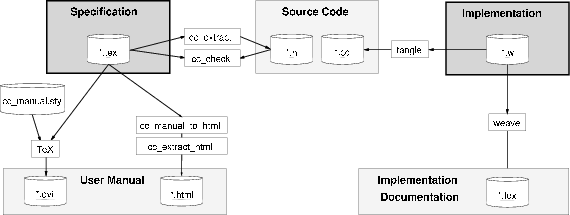
\includegraphics[width=1.0\textwidth]{Manual_tools/tools_overview}%
    \caption{The files and tools involved in the manual writing
      process.\index{files}\index{tools}}}
    \label{ToolsOverviewFig}\figuretopindent
\begin{ccHtmlOnly}
<CENTER>
  <IMG SRC="Manual_tools/tools_overview.gif" ALT="Files and tools used in manual writing">
</CENTER>
\end{ccHtmlOnly}
\end{figure}

\index{naming scheme} The style uses a {\tt cc} prefix\index{name
  prefix} for its macros since it is related to format \CC\
declarations. The only exceptions are the common abbreviations listed
in the next section. Their usefulness is their brevity. The naming
scheme requires macro names in lower case.  Concatenated names start
with an upper case letter, for example, \verb+\ccFunction+.

\index{layout} The formatting is closely related to that of the
LEDA\TTindex{LEDA} manual \cite{Naeher95}.  More precisely, a manual
page is structured with subtitles followed by main text blocks and
declarations. A declaration is formatted in a \Dindex{three-column
  layout} with certain flexibilities.  The first column contains the
type of a variable or the return type of a function. The second column
contains the variable name or the function name with its argument
list. The third column contains an optionally empty description for
that declaration. This way, a short member function can be efficiently
documented in one line. The widths of the columns are fixed but
customizable at any time. If an entry exceeds the reserved space in
its column, it expands to the next columns forcing the remaining
entries to start in the next line. The description in the third column
is block formatted.  Declarations, such as constructors or enums, set
their first column to zero width, thus behaving like a two-column
formatting.  A specialty are too long \Dindex{item lists}.  They are
formatted one item per line, for example, long function argument lists
or enum values. A couple of advanced macros are available for further
customization of the layout. The following is an example of the
layout: \index{argument lists}\index{parameter lists}

\ccSetThreeColumns{int bla}{foo blabla( double d)}{}
\lcTex{\ccwIndent=10mm}
\ccFunction{int foo( double d);}{returns an integer from wherever.}
\lcTex{\ccwIndent=0mm}


% ----------------------------------------------------------------------
\section{Including \CC\ source code}
\label{sectionSourceCode}
\index{C++ source code, including@\CC\ source code, including}


The style {\tt cprog.sty} offers a macro \verb+\cprogfile{+{\em
filename\/}\verb+}+ to include C source code files verbatim into
the document, but with font changes for C comments and such. However,
\CC\ source code is not well supported. Similar to the {\tt verbatim}
environment, the {\tt ccExampleCode} environment encapsulates source
code examples. The related \verb+\ccIncludeExampleCode{+{\em
filename\/}\verb+}+ command includes and formats source code
files. License headers in example source files are stripped and
a filename is printed below the example code.

The macro \verb+\ccIncludeVerbatim{+{\em filename\/}\verb+}+
includes a file verbatim without any further formatting and displays
it in {\tt tt}-style.
\ccIndexEntry{IncludeVerbatim}\ccIndexEntry{IncludeExampleCode}\TTindex{cprog.sty}
\TTindex{cprogfile}\index{example source code}
\Eindex{ccExampleCode}

\begin{tabbing}
\lcTex{ M \= \kill}
 \> \verb+\begin{ccExampleCode}+ {\em source code} \verb+\end{ccExampleCode}+\\
 \> \verb+\ccIncludeExampleCode{+{\em filename}\verb+}+\\
 \> \verb+\ccIncludeVerbatim{+{\em filename}\verb+}+
\end{tabbing}

\section{Revision data}
\label{sectionRCSmacros}
\index{revision number}

The revision control system \Dindex{SVN} manages variables like the
revision number or date within \$-symbols in source files. The macro
\verb+\RCSdef{+{\em macro\/}\verb+}{+{\em RCSentry\/}\verb+}+ assigns
the RCS variable contents in {\em RCSentry\/} to the given {\em
  macro\/} without the enclosing \$-symbols. The macro
\verb+\RCSdefDate{+{\em macro\/}\verb+}{+{\em RCSdate\/}\verb+}+ is
specialized for the date entry of RCS. It extracts the date and
assigns it to the given {\em macro}. The time which is also part of
the RCS date entry is omitted.  The revision number and the date of
the revision of the {\tt cc\_manual.sty} are available with the macros
\verb+\ccRevision+ and\verb+\ccDate+.
\ccIndexEntry{Revision}\ccIndexEntry{Date}\index{RCS revision of style}
\index{RCS date of style}\index{date extraction for RCS}

\RCSdef{\aManual}{$Id$}
\RCSdefDate{\bManual}{$Date$}

\begin{scriptsize}
\begin{tabbing}
\lcTex{  M \= implementationNNN \= ImplementationMMMMM \= \kill}
  \> \verb@\RCSdef{\a}{$Id$}@ \hspace*{1cm}\=\\
  \> \verb@\RCSdefDate{\b}{$Date$}@ \\
  \> \verb+\a+ \>       \aManual \\
  \> \verb+\b+ \>       \bManual \\
  \> \verb+\ccRevision+ \> \ccRevision \\
  \> \verb+\ccDate+     \> \ccDate
\end{tabbing}\Mindex{RCSdef}\Mindex{RCSdefDate}
\end{scriptsize}

\section{Common Abbreviations}
\label{sectionCommonAbbrev}
\index{common abbreviations}\index{abbreviations, common}

The abbreviations for the number set symbols in blackboard bold math
need the package {\tt amssymb} and \LaTeXe.

\begin{tabbing}
\lcTex{  M \= dummyyyyyyyy \= kjdshfksdjfhksjdfhkjdhfijdfsdf \= dummyMMM \= \kill}
  \> \verb+\CC+         \> \CC         \> \verb+\N+        \> \N\\
  \> \verb+\gcc+        \> \gcc        \> \verb+\Z+        \> \Z\\
  \> \verb+\nat+        \> \nat        \> \verb+\Q+        \> \Q\\
  \> \verb+\real+       \> \real       \> \verb+\R+        \> \R\\
  \> \verb+\cgal+       \> \cgal       \> \verb+\E+        \> \E\\
  \> \verb+\galia+      \> \galia      \> \verb+\leda+     \> \leda\\
  \> \verb+\stl+        \> \stl        \> \verb+\plageo+   \> \plageo\\
  \> \verb+\protocgal+  \> \protocgal
\end{tabbing}
\Mindex{CC}\Mindex{gcc}\Mindex{nat}\Mindex{real}
\Mindex{leda}\Mindex{cgal}\Mindex{galia}
\Mindex{protocgal}\Mindex{plageo}\Mindex{N}\Mindex{Z}\Mindex{Q}\Mindex{R}
\Mindex{E}


% ----------------------------------------------------------------------
\section{Structuring Macros}
\label{sectionStructureMacros}

The macro \verb+\ccChapterSubTitle{+{\em text\/}\verb+}+ formats a
subtitle {\em text\/} for a chapter in a small italics font.  Multiple
\verb+\ccChapterSubTitle+ macros are possible.  Two similar macros,
\verb+\ccChapterAuthor+ and \verb+\ccChapterRelease+, provide
formatting for chapter authors or a release number\footnote{This is
  useful for a multi-author manual or an RCS release number or date
  as it is available with the \Backslash {\tt RCSdef} or \Backslash {\tt
    RCSdefDate} macros from Section~\ref{sectionRCSmacros}.}.

All macros are formatted in \TeX\ vertical mode. They can be used
several times and in arbitrary order, with or without paragraphs (that
will be ignored in formatting them). They should be placed right after
the chapter macro.

The \verb+\ccChapterAuthor+ macro is intended for formatting chapter
authors. One macro call suffices to format all authors of one
chapter. The authors are, for example, given in alphabetical order and
separated by \verb+\and+ macros, which then expand properly to commas
and a ``, and'' text. White space surrounding the \verb+\and+ macros
is eliminated. One can use the \verb+\\+ control sequence to enforce a
line break, but only in the macro argument, not outside of the macro,
since there  we are in \TeX\ vertical mode.

The author macro is active and the release macro is inactive by
default (since the official \cgal\ manual is written this way), but
they can be activated and deactivated using the boolean values
\verb+\ccTagChapterAuthor+ and \verb+\ccTagChapterRelease+, as
described in Section~\ref{sectionCustomizeMisc}. The example assumes
both values set to \verb+\ccTrue+ and the manual release in \verb+\a+
and the manual date in \verb+\b+.
\ccIndexEntry{ChapterSubTitle}\index{subtitle of a chapter}
\ccIndexEntry{ChapterAuthor}\ccIndexEntry{ChapterRelease}
\ccIndexEntry{TagChapterAuthor}\ccIndexEntry{TagChapterRelease}
\index{author|see{\Backslash{\tt ccChapterAuthor}}}
\index{release|see{\Backslash{\tt ccChapterRelease}}}
\index{revision|see{\Backslash{\tt ccChapterRelease}}}
\index{and|\Backslash{\tt and}}

\begin{tabbing}
\lcTex{  M \= \hspace*{94mm} \= \kill}
  \> \verb+\ccChapterSubTitle{String}+      \>  {\em String}\\
  \> \verb+\ccChapterRelease{\a, \b}+       \>  {\em \aManual, \bManual}\\
  \> \verb+\ccChapterAuthor{Alt}+           \>  {\em Alt}\\
  \> \verb+\ccChapterAuthor{Alt \and Jung}+ \>  {\em Alt and Jung}\\
  \> \verb+\ccChapterAuthor{Alt \and Jung \and J\"unger}+
                                            \>  {\em Alt, Jung, and J\"unger}
\end{tabbing}

The name of a class that is defined in a section or subsection might
appear in its title.  The following two macros act like the normal
\verb+\section+ or \verb+\subsection+ macros with the classname
appended in parenthesis.  Precondition is that a classname is known in
the current scope, i.e.\ that we are within a \verb+ccClass+ or
\verb+ccClassTemplate+ environment as described in
Section~\ref{sectionClass}. Note that the macro \verb+\ccClassName+
will not work properly without protection and consideration of the
table-of-contents.  For the following example we assume a classname
\verb+Armadillo+ here.

\begin{tabbing}
\lcTex{  M \= \hspace*{77mm} \= \kill}
  \> \verb+\ccSection{Title}+        \> {\Large\bf 2 Title ({\it Armadillo})}\\
  \> \verb+\ccSubsection{Subtitle}+  \> {\bf 2.1 Subtitle ({\it Armadillo})}
\end{tabbing}
\ccIndexEntry{Section}\ccIndexEntry{Subsection}


The following abbreviations for subsections are not numbered.  They
are intended to structure the main text in the given order. Empty
subsections are possible (therefore no numbering).

\begin{tabbing}
\lcTex{  M \= CCimplementationNNN \= IsxModelxforxthexConceptxxx \= \kill}
  \> \verb+\ccDefinition+      \>  {\bf Definition}    \>
                                          including template parameters\\
  \> \verb+\ccInheritsFrom+    \>  {\bf Inherits From}     \>
                                                     base classes\\
  \> \verb+\ccHasModels+       \>  {\bf Has Models}     \>
                                                     models for concepts\\
  \> \verb+\ccIsModel+         \>  {\bf Is Model for the Concept}     \>
                                                     concept names\\
  \> \verb+\ccGeneralizes+     \>  {\bf Generalizes}     \>
                                                     concept names\\
  \> \verb+\ccRefines+         \>  {\bf Refines}     \>
                                                     concept names\\
  \> \verb+\ccRequirements+    \>  {\bf Requirements}     \>
                                                     type requirements, etc.\\
  \> \verb+\ccTypes+           \>  {\bf Types}         \>
                                                     local type definitions \\
  \> \verb+\ccConstants+       \>  {\bf Constants}     \>
                                                     constant values\\
  \> \verb+\ccCreation+        \>  {\bf Creation}      \>
                                                     constructors, assignment\\
  \> \verb+\ccOperations+      \>  {\bf Operations}    \>
                                                     functions and operators\\
  \> \verb+\ccAccessFunctions+ \>  {\bf Access Functions}    \>
                                                     member access\\
  \> \verb+\ccQueryFunctions+ \>   {\bf Query Functions}    \>
                                                     query functions\\
  \> \verb+\ccPredicates+      \>  {\bf Predicates}    \>
                                                     predicates\\
  \> \verb+\ccModifiers +      \>  {\bf Modifiers}    \>
                                                     insert, delete, update\\
  \> \verb+\ccSeeAlso+         \>  {\bf See Also}\>
                                                     other classes, functions\\
  \> \verb+\ccImplementation+  \>  {\bf Implementation}\>
                                                     running time, memory\\
  \> \verb+\ccExample+         \>  {\bf Example}       \>
                                                     programming examples
\end{tabbing}
\ccIndexEntry{Definition}\ccIndexEntry{InheritsFrom}\ccIndexEntry{Constants}
\ccIndexEntry{Types}\ccIndexEntry{Creation}\ccIndexEntry{Operations}
\ccIndexEntry{AccessFunctions}\ccIndexEntry{Predicates}\ccIndexEntry{Modifiers}
\ccIndexEntry{SeeAlso}\ccIndexEntry{Implementation}\ccIndexEntry{Example}
\ccIndexEntry{HasModels}\ccIndexEntry{IsModel}\ccIndexEntry{Generalizes}
\index{base class}\index{concept model}

An additional title not mentioned here can be formatted with
\verb+\ccHeading{...}+. For example the subsection on operations might
get split up for larger classes in more specific parts as access
functions, predicates, and modifiers, also predefined titles listed above.
Necessary include files go at the end of the definition part. Multiple
includes should be separated with \verb+\\+.
\ccIndexEntry{Heading}\ccIndexEntry{Include}\index{header files}

\begin{tabbing}
\lcTex{  M \= CCimplementationNNNMMMMMMMMMMM \= \kill}
  \> \verb+\ccInclude{CGAL/Vector_2.h}\\+\>  \ccc{#include <CGAL/Vector_2.h>}\\
  \> \verb+\ccInclude{CGAL/Point_2.h}+   \>  \ccc{#include <CGAL/Point_2.h>}
\end{tabbing}


A few subtitles are predefined for the descriptive text in the third
column.

\begin{tabbing}
\lcTex{  M \= CCimplementationNNN \=\kill}
  \> \verb+\ccPrecond+       \>  {\it Precondition}: \\
  \> \verb+\ccPostcond+      \>  {\it Postcondition}: \\
  \> \verb+\ccRequire+       \>  {\it Requirement}:
\end{tabbing}
\ccIndexEntry{Precond}\ccIndexEntry{Postcond}

A {\em precondition\/} is an expressions that evaluates to {\tt true}
at the entry point of a function or constructor call. As long as it is
not explicitly switched off during compilation, the functions are
supposed to check these preconditions at run time if it is possible in
feasible time. A {\em postcondition\/} is an expression that evaluates
to {\tt true} at the exit point of a function or constructor call and
is likewise supposed to be checked. Roughly spoken, the precondition
protects the function against user errors, the postcondition protects
the user against programming errors in the function. Program
checkers \cite{Mehlhorn96} fall in the category of postconditions.

\begin{ccAdvanced}
An additional entry can be formatted with
\verb+\ccCommentHeading{...}+.

\begin{tabbing}
\lcTex{  M \= CCimplementationNNNMMMMMMMM \= ImplementationMMMMM \= \kill}
  \> \verb+\ccHeading{Text}+         \> {\bf Text}\\
  \> \verb+\ccCommentHeading{Text}+  \> {\it Text}:
\end{tabbing}
\ccIndexEntry{Heading}\ccIndexEntry{CommentHeading}

Advanced sections in the reference manual can be marked  with the environment
\verb+\begin{ccAdvanced} ... \end{ccAdvanced}+. The environment
produces angles around the encapsulated paragraphs like it does here.
%\index{ccadvanced environment@{\tt ccAdvanced} environment}
\Eindex{ccAdvanced}
\end{ccAdvanced}

% ----------------------------------------------------------------------
\section{Multiple Manuals in One Document}
\label{sectionPartCommand}

The \LaTeX\ \verb+\part+\lcIndex{part} command can be used to generate a
single document that consists of more than one manual but has a common table
of contents, index and bibliography.  This can be used, for example, to
combine a user manual and reference manual and thus get easy referencing
between the two while keeping them logically separated.  The command
\verb+\ccNumberChatpersByPart+ should be used if you wish to start renumbering
chapters at 1 after each new \verb+\part+ command (which is probably a
good idea); otherwise chapter numbering is continuous.
For the HTML conversion, the command \verb+\ccMultiplePartsToc+ should be used
to tell the HTML converter to use the appropriate format for the table of
contents.

For manuals written with separate user and reference manual parts it is
useful to have a link between a chapter in the user manual part and its
corresponding chapter in the reference manual, and vice versa.  The
macros \verb+\ccUserChapter+ and \verb+\ccRefChapter+ are provided to
produce this in the HTML manual.  These macros act as substitutes for the
\verb+\chapter+ command (and are synonyms for this in the \LaTeX\ style
file), but take two arguments instead of one. The first argument is the
title of the chapter and the second is the label for the corresponding
chapter to which a link is to be created.
\ccIndexEntry{UserChapter}\index{reference manual, crosslink to}
\ccIndexEntry{RefChapter}\index{user manual, crosslink to}


% ----------------------------------------------------------------------
\section{\CC\ Formatting}

All arguments of macros that are \CC\ code are parsed from \TeX\ with
changed \verb"\catcode"\index{catcode} values for some characters.
This allows to use such \Dindex{special characters} as ``\_'' in \CC\
declarations without quoting them as it is usual within \LaTeX.  The
rule is that in any case, the complete original \CC\ source text is
written without quoting. The formatting macros handle for example the
special characters \_, {\tt <}, {\tt >}, and {\tt \&} as they appear
in \CC\ names and the characters \#, \%, \ccHat, and \ccTilde\ as they
appear with operators and the preprocessor. The macro
\verb+\ccStyle{+{\em src\/}\verb+}+ (abbr.\ \verb+\ccc+) does this
formatting for a given \CC\ source code {\em
  src}.\ccIndexEntry{c}\ccIndexEntry{Style} But, for example, \TeX\ comments
with the leading ``\%'' sign will not work within the \CC\ code.

\begin{tabbing}
\lcTex{  M \= CCimplementationNNMNMMMMMMMMMM \= ImplementationMMMMM \= \kill}
  \> \verb+\ccStyle{A f_bar(X<T>& x = "%^~#");}+
        \>  \ccStyle{A f_bar(X<T>& x = "%^~#");}\\
  \> \verb+\ccc{A f_bar(X<T>& x = "%^~#");}+
        \>  \ccc{A f_bar(X<T>& x = "%^~#");}
\end{tabbing}
\ccIndexEntry{Style}\ccIndexEntry{c}

Several of the following macros have multiple parameters. Only the
parameters that should contain \CC\ code are parsed with the changed
catcodes\index{catcode}. The catcodes are restored right after the
closing braces of these parameters.  An unavoidable side effect of the
\TeX\ character scanner is that these changed catcodes will not apply
if these macros are used itself within the argument of another macro.
In that case, the argument's text is just once scanned by \TeX\ when
reading the outer argument up to the end of its scope, and the changing of
the catcodes applies too late for the scanning process of \TeX. Without
going into unnecessary details here, the macros of this package will
nonetheless (most probably) work fine as long as no special characters
occurs.  In any circumstances, these macros work with environments or
braces used for grouping.

% ----------------------------------------------------------------------
\section{\CC\ Reference Pages}
\label{sectionRefPages}\index{reference pages, \CC}\index{reference manual}

Each class, concept, function, etc., is documented in an environment.
For the purpose of the supporting tools, e.g., the HTML converter,
each of them is best put in its own file. The environments have a
single parameter for the item name. For the item name, only the
identifier plus an optional list of template arguments (for classes)
is given. Function parameters, function template declarations or macro
parameters or not given here. The item name will be formatted as
section title. Member declarations of concepts and classes and the
global declarations for enums, variables, constant, functions and macros
are written within these environments using the macros following in the
sections below. The currently available environments are:

\begin{tabbing}
\lcTex{\= CCimplementationNNNMMMMMMMMMMMn \= Imple \= \kill}
  \> \verb+\begin{ccRefConcept}{Circulator}+ \> {\em text}
  \> \verb+\end{ccRefConcept}+\\
  \> \verb+\begin{ccRefFunctionObjectConcept}{C}+ \> {\em text}
  \> \verb+\end{ccRefFunctionObjectConcept}+\\
  \> \verb+\begin{ccRefClass}{Circulator_traits<C>}+ \> {\em text}
  \> \verb+\end{ccRefClass}+\\
  \> \verb+\begin{ccRefFunctionObjectClass}{C<R>}+ \> {\em text}
  \> \verb+\end{ccRefFunctionObjectClass}+\\
  \> \verb+\begin{ccRefEnum}{Orientation}+ \> {\em text}
  \> \verb+\end{ccRefEnum}+\\
  \> \verb+\begin{ccRefFunction}{is_empty_range}+ \>{\em text}
  \> \verb+\end{ccRefFunction}+\\
  \> \verb+\begin{ccRefVariable}{VARIABLE}+ \> {\em text}
  \> \verb+\end{ccRefVariable}+\\
  \> \verb+\begin{ccRefConstant}{ORIGIN}+ \> {\em text}
  \> \verb+\end{ccRefConstant}+\\
  \> \verb+\begin{ccRefMacro}{For_all}+ \> {\em text}
  \> \verb+\end{ccRefMacro}+
\end{tabbing}
\Eindex{ccRefConcept}
\Eindex{ccRefClass}
\Eindex{ccRefEnum}
\Eindex{ccRefFunction}
\Eindex{ccRefFunctionObjectClass}
\Eindex{ccRefFunctionObjectConcept}
\Eindex{ccRefVariable}
\Eindex{ccRefConstant}
\Eindex{ccRefMacro}
\index{function object|see{{\tt ccRefFunctionObjectConcept}}}
\index{function object!class|see{{\tt ccRefFunctionObjectClass}}}
\index{concept|see{{\tt ccRefConcept}}}\index{class|see{{\tt ccRefClass}}}
\index{enum|see{{\tt ccRefEnum}}}\index{function|see{{\tt ccRefFunction}}}
\index{variable|see{{\tt ccRefVariable}}}\index{macro|see{{\tt ccRefMacro}}}

These environments have an optional argument to declare a
\Dindex{class scope} or \Dindex{namespace} that the item is in.
Furthermore, the style maintains a \Dindex{global scope}, which is
prepended to each item except {\tt Concept}, {\tt FunctionObjectConcept}
and {\tt Macro}.\index{scope, class}\index{scope, global}. The global scope
is empty by default.

\begin{tabbing}
\lcTex{  M \= CCimplementationNNNMMMMMMMMM \= ImplementationMMMMM \= \kill}
  \> \verb+\ccDefGlobalScope{CGAL::}+    \>   \\
  \> \verb+\begin{ccRefConcept}{Circulator}+
    \> {\large\bf Concept Circulator}  \\
  \> \verb+\end{ccRefConcept}+ \\
  \> \verb+\begin{ccRefClass}[Poly::]{Vertex}+
    \> {\large\bf Class CGAL::Poly::Vertex}\\
  \> \verb+\end{ccRefClass}+
\end{tabbing}
\ccIndexEntry{DefGlobalScope}

There are two different styles of formatting the reference pages. The
old style created a section title as in the example above. The new
style, which is now the default choice, creates a new page for each
item and draws a tab marker at
the side margin indicating the category of this item. Use the
\verb+\ccNewRefManualStyle+ macro as follows to switch between these
styles explicitly. The tab markers use the side margins of \LaTeX. The
dimensions of the side margins need to be set accordingly.
\ccIndexEntry{NewRefManualStyle}\Mindex{marginparsep}\Mindex{marginparwidth}

\begin{tabbing}
\lcTex{  M \= CCimplementationNNNMMMMMMMMM \= ImplementationMMMMM \= \kill}
  \> \verb+\marginparsep7mm+\\
  \> \verb+\marginparwidth15mm+\\
  \> \verb+\gdef\ccNewRefManualStyle{\ccTrue}+
\end{tabbing}

The macro \verb+\ccRefPageBegin+\ccIndexEntry{RefPageBegin} is called
just before the section title of a reference page is formatted. The
macro \verb+\ccRefPageEnd+\ccIndexEntry{RefPageEnd} is called after
all formatting of the reference page is finished.  These two macros
are user-customizable and empty by default. The following redefinition
of these macros places each reference page on its own page. Note that
this redefinition is superfluous if the second style for reference
pages has been selected.

\begin{tabbing}
\lcTex{  M \= CCimplementationNNNMMMMMMMMM \= ImplementationMMMMM \= \kill}
  \> \verb+\renewcommand{\ccRefPageBegin}{\clearpage}+ \\
  \> \verb+\renewcommand{\ccRefPageEnd}{\clearpage}+
\end{tabbing}

\index{page breaks!turning off}
The macro \verb+\ccRefPageBreak+\ccIndexEntry{RefPageBreak} can be used to
turn off and on the page breaks that occur at the beginning an end of each
\verb|ccRef*| section.  For example, the following set of commands
will suppress the page break that normally occurs at the end of a
\verb|ccRefConcept| environment in the new manual style:

\begin{tabbing}
\lcTex{  M \= CCimplementationNNNMMMMMMMMM \= ImplementationMMMMM \= \kill}
  \> \verb+\gdef\ccNewRefManualStyle{\ccTrue}+ \\
  \> ...  \\
  \> \verb+\begin{ccRefConcept}+ \\
  \> \VarText{concept description} \\
  \> \verb+\gdef\ccRefPageBreak{\ccFalse}+ \\
  \> \verb+\end{ccRefConcept}+
\end{tabbing}

For object declarations and member functions we use a variable name
{\em var\/} for the object defined with the
\verb+\ccCreationVariable{+{\em var\/}\verb+}+ macro. It must not be
used outside of these environments and it is a precondition for the
\verb+\ccConstructor{+\ldots\verb+}{+\ldots\verb+}+ or
\verb+\ccMemberFunction{+\ldots\verb+}{+\ldots\verb+}+ macros, see
below. The variable name can but usually does not change within a
class declaration.

\begin{tabbing}
\lcTex{  M \= CCimplementationNNNMMMMMMMM \= ImplementationMMMMM \= \kill}
  \> \verb+\ccCreationVariable{g}+
\end{tabbing}
\ccIndexEntry{CreationVariable}
\ccCreationVariable{g}

The variable name, the parameters given to the environment, and the
global scope are available in the environment using the following
macros. They are grouped into the already formatted names and the
non-formatted names (the parameters originally given without font
specifications).  The following table shows the different
possibilities assuming we are in the class example from above for the
class \ccc{CGAL::Poly::Vertex}.

\begin{tabbing}
\lcTex{  M \= ccClassTemplateName \= \ccClassTemplateName MMMMMMMM
      \= CCpuretemplatenameMMMM \= \kill}
  \>formatted  \> example \> unformatted ~~~~~~~~~~~~
                 example using \verb+\tt+\\[1ex]
  \>\> \> \verb+\ccRefCategory+  \> {\tt Class}\\
  \>\verb+\ccGlobalScope+  \> \ccc{CGAL::}
    \> \verb+\ccPureGlobalScope+ \> {\tt CGAL::}  \\
  \>\verb+\ccRefScope+  \> \ccc{Poly::}
    \> \verb+\ccPureRefScope+ \> {\tt Poly::}  \\
  \>\verb+\ccRefName+ \> \ccc{Vertex} \> \verb+\ccPureRefName+ \>{\tt Vertex}\\
  \>\verb+\ccVar+ \> \ccVar \> \verb+\ccPureVar+ \> {\tt\ccPureVar}
\end{tabbing}
\ccIndexEntry{RefCategory}\ccIndexEntry{GlobalScope}
\ccIndexEntry{PureGlobalScope}\ccIndexEntry{RefScope}
\ccIndexEntry{PureRefScope}\ccIndexEntry{RefName}
\ccIndexEntry{PureRefName}\ccIndexEntry{Var}\ccIndexEntry{PureVar}

Each reference page environment declares automatically a label for its
current position. The label is named \verb+\ccRef_+{\em itemname}.
Note that the section titles created with these environments are not
numbered. Thus, the labels can be used only for page references. For
convenience, the following macros allow one to define additional
labels, \verb+\ccRefLabel{+{\em idfier}\verb+}+, and to create page
references, \verb+\ccRefPage{+{\em idfier}\verb+}+. The macros
\verb+\ccRefIdfierPage{+{\em idfier}\verb+}+ and
\verb+\ccRefConceptPage{+concept\verb+}+ help to build a kind of
table-of-contents listing of several identifiers that can be useful in
an introduction section placed before the collection of the reference
pages. The macro \verb|\ccRefIdfierPage| should be used for all reference pages
labeled with \CC\ identifiers ({\em i.e.}, for everything except concepts);
\verb|\ccRefConceptPage| should be used for concepts.
The macros format their arguments in the usual way and
create page references.

You can change the way these page references are formatted using the
commands \verb+\ccRefPageNumAtMargin+\ccIndexEntry{RefPageNumAtMargin} and
\verb+\ccRefPageFill+\ccIndexEntry{RefPageFill}.  If the first
command is set to \verb+\ccTrue+ (the default), page numbers are printed
at the right margin with the space in between filled using
\verb+\ccRefPageFill+.  The default value for \verb+\ccRefPageFill+
is \verb+\dotfill+.  When \verb+\ccRefPageNumAtMargin+  is set to
\verb+\ccFalse+, page numbers appear directly after the identifiers in
parentheses using the format ``(pg. \#)''.  Note that the \LaTeX\
to HTML converter ignores these page references since it expects to
generate proper hyper-links for the identifier used as the
argument for \verb+\ccRefIdfierPage+ or \verb|\ccRefConceptPage|.
If you want the page reference
to appear in the HTML manual as well, use the usual \verb+\pageref+
macro with the full name of the label.


\ccRefLabel{ClassA}\ccRefLabel{ClassB}
\ccRefLabel{A_Concept}
\begin{tabbing}
\lcTex{  M \= CCimplementationNNNMMMMMMMMMM \= ImplementationMMMMM \= \kill}
  \> \verb+\ccRefLabel{ClassA}\ccRefLabel{ClassB}\ccRefLabel{A_Concept}+ \\ ~\\
  \> see for example \verb+\ccRefPage{ClassA}+.\verb+\\+
      \> see for example \ccRefPage{ClassA}.\\
  \> \verb+\ccRefIdfierPage{ClassA}\\+ \> \ccc{ClassA} \> \ccRefPage{ClassA}\\
  \> \verb+\ccRefIdfierPage{ClassB}+ \> \ccc{ClassB} \> \ccRefPage{ClassB}\\
  \> \verb+\ccRefConceptPage{A_Concept}+ \> A\_Concept \> \ccRefPage{A_Concept}
\end{tabbing}
\ccIndexEntry{RefPage}\ccIndexEntry{RefLabel}\ccIndexEntry{RefIdfierPage}
\ccIndexEntry{RefConceptPage}


Some useful tools are available that help in writing and organizing
reference pages. The {\tt cc\_ref\_wizard} script generates reference
page templates. It expects the category of reference page and the item
name. The {\tt cc\_make\_ref\_pages} script creates a {\tt main.tex}
file for a subdirectory of reference pages. The resulting file
includes all {\tt *.tex} files in a subdirectory in alphabetical
order. If a file called {\tt intro.tex} exists it is included first.
This file is supposed to give some chapter title, some introduction,
and an overview of the reference pages, for example, a
table-of-contents created with the \verb+\ccRefIdfierPage+ and
\verb+\ccRefConceptPage+ macros from above. Both scripts give a list
of options if called without
parameters. An example of reference pages is given in the {\tt example}
subdirectory of the distribution of this style file and its related
tools.\TTindex{cc\_make\_ref\_pages}\TTindex{cc\_ref\_wizard}
\index{example reference pages}\index{reference pages, example}
\index{scripts cc\_make\_ref\_pages@scripts, {\tt
    cc\_make\_ref\_pages}} \index{scripts, cc\_ref\_wizard@scripts,
  {\tt cc\_ref\_wizard}}

The command \verb+\listofrefpages+\lcIndex{listofrefpages} is similar to
the \verb+\listoffigures+
and \verb+\listoftables+ commands provided with \LaTeX.  It produces a file
with extension \texttt{.ref} containing a list of all reference pages.  When
\LaTeX\ is run again, this list of pages will be placed at the point where
the \verb+\listofrefpages+ command occurs in the source file.  To get an
alphabetical listing of these pages you need only sort the \texttt{.ref}
file by the appropriate key using, for example, the Unix sort command before
running \LaTeX.  This command currently has no effect in the HTML conversion.


% ----------------------------------------------------------------------
\section{\CC\ Declarations}
\label{sectionDeclarations}
\index{declarations} \index{C++ declarations@\CC\ declarations}

We use macros to distinguish different types of declarations, for
example constructors, functions, and member functions, also called
{\em methods}.

One group is designed to specify class member declarations, another is
derived therefrom to specify global declarations like global functions
or enums. Class declarations tend to have lots of small member
functions and operations, where the three-column layout is well suited
to fully document a declaration in the third column. For global
declarations the documentation tends to be longer and is better placed
in the main text above or below the declaration. Here the third column
remains empty. All class member declarations can also be used for
global declarations where the description in the third column seems
appropriate (with the exceptions of
\verb+\ccMemberFunction{...}{...}+ and \verb+\ccConstructor{...}{...}+).
\index{global declarations}\index{three-column layout}
\index{two-column layout|see{three-column}}

\index{layout} \index{reduction rules} \index{simplification rules}
\index{rules|see{reduction rules}} \index{formatting} \index{operator
  formatting} \index{const ref@{\tt const \ldots \&} removal}
\index{argument list formatting} \index{parameter|see{argument}}
\index{cast operator} \index{operator()@{\tt operator()({\em
      args\/})}} \index{operator type@{\tt operator {\em type\/}()}}
Several rules are built in to simplify the appearance of \CC\
declarations in the manual. By default they are all active, but they
can be switched off separately, see Section~\ref{sectionCustomize}.
The first rule examines function argument lists for
call-by-constant-reference parameters, {\tt const \ldots \&}, and
removes the const-reference modifier. Const-reference parameters are a
matter of efficiency and are almost always semantically equivalent to
call-by-value parameters~\footnote{In cases where const-reference
  parameters make a difference to call-by-value parameters, it has to
  be documented explicitly anyway. An option is provided later on to
  show then the const-reference modifier.}. The second rule examines
the argument lists for types that are equal to the classname in the
current environment and removes these types. The results are short and
very readable copy constructors, assignments, and operator notations.
The third rule detects operator declarations, either as functions or
as member functions, and formats them in operator notation. All
operators that can be overloaded by \CC\ are handled, including the
{\tt operator()(}{\em args\/}{\tt )} with any number of arguments {\em
  args} and the cast operator {\tt operator {\em type\/}()}.  The
fourth rule removes all parts of a function, member function, or
constructor that follow the closing parenthesis. This is intended for
the {\tt const} modifier for member functions. The following example
uses several macros from the next section to illustrate the
simplification rules. The formatting principle behind these rules is
to show the usage of a certain function, type, or variable enriched
with type informations where necessary. This implies for member
functions the usual dot notation and that the trailing {\tt const} is
not visible.

\begin{tabbing}
\lcTex{  M \= MM\= CCimplementationNNNMMMMMMMMMMMMM \= intN \= foo(coXx);MM \=\kill}
  \> \verb+\begin{ccClass}{A}+\>\>{\em formatting result}:\\
  \>\> \verb+\ccCreationVariable{a}+\\
  \>\> \verb+\ccFunction{int foo(const X& x);}{+\ldots\verb+}+
    \> \ccStyle{int}  \> \ccStyle{foo(X x)}  \>  \ldots \\
  \>\> \verb+\ccFunction{A foo(const A& c);}{+\ldots\verb+}+
    \> \ccStyle{A}  \> \ccStyle{foo(c)}  \>  \ldots \\
  \>\> \verb!\ccFunction{A operator+(A a, A b);}{!\ldots\verb+}+
    \> \ccStyle{A}  \> \ccStyle{a + b}  \>  \ldots \\
  \>\> \verb!\ccMethod{A operator+(A b);}{!\ldots\verb+}+
    \> \ccStyle{A}  \> \ccStyle{a + b}  \>  \ldots \\
  \>\> \verb+\ccMethod{int bar() const;}{+\ldots\verb+}+
    \> \ccStyle{int}\> \ccStyle{a.bar()}  \>  \ldots \\
  \> \verb+\end{ccClass}+
\end{tabbing}
\ccIndexEntry{Section}\ccIndexEntry{Subsection}

Three macros deal with the interplay between the specification and
implementation. \verb+\ccDeclaration{+{\em decl\/}\verb+}+ and
\verb+\ccHidden+ allow to incorporate \CC\ declarations {\em decl\/}
in the manual that are not printed but that are checked by the {\tt
  cc\_check}\TTindex{cc\_check} tool. This is for example useful in
the case where a {\tt const} and a non-{\tt const} version of a member
function exists, so that they are indistinguishable in the manual, but
both are necessary in the implementation. \verb+\ccHidden+ is a kind
of modifier. When it is prepended to one of the declaration macros
below with two parameters (one for the \CC\ declaration and one for
the comment), this declaration is no longer shown in the manual but
checked against the implementation. The third macro
\verb+\ccUnchecked+ works the other way around. The declaration
remains in the manual, but it is excluded from the check with the {\tt
  cc\_check} tool. This is useful if the visible declaration in the
manual does not tell the whole truth. An example are proxies which one
does not want to expose in the manual.

\begin{tabbing}
\lcTex{  M \= CCimplementationNNNMMMMMMMMMMMMMMMM \= ImplementationMMMMM \= \kill}
  \> \verb+\ccDeclaration{int x;}+    \>   \\
  \> \verb+\ccHidden\ccVariable{int x;}{superfluous.}+    \>   \\
  \> \verb+\ccUnchecked\ccVariable{int y;}{comment.}+    \>
  {\it int y;}\ \ \ \ comment.
\end{tabbing}
\ccIndexEntry{Style}



% ----------------------------------------------------------------------
\begin{ccClassTemplate}{Gnu<T>}
\ccSection{Class and Class Member Declarations}
\label{sectionClass}

\index{class members}
\index{members|see{class members}}
%\index{ccClass environment@{\tt ccClass} environment}
\Eindex{ccClass}
\index{template, class|see{{\tt ccClassTemplate}}}
%\index{ccClassTemplate environment@{\tt ccClassTemplate} environment}
\Eindex{ccClassTemplate}

A class is declared with a {\tt ccClass} environment. The environment
has a single parameter that contains the name of the class. The member
declarations for the class are written within this environment.  A
class template is similarly declared with a {\tt ccClassTemplate}
environment.  The environment parameter contains the class name
including its template parameters. These template parameters must be
the same when used for example for an argument in a function parameter
list. Otherwise the automatic removal of the class name from an
argument list will not work, see Section~\ref{sectionRulesSimple} for
details. Note that a \Dindex{nested class} {\tt B} like in {\tt
  A<T>::B} is {\em not} a class template. The {\tt ccClass}
environment must be used in this case.

Within these class defining environments exist a set of macros that
stand for the current name of the class and the current template
parameters, see below.  These names are the precondition for the
\verb+\ccSection+ and \verb+\ccSubsection+ macros from
Section~\ref{sectionStructureMacros}. The section title above is an
example of the {\tt ccClassTemplate} environment followed by a
\verb+\ccSection+.

\begin{tabbing}
\lcTex{  M \= CCimplementationNNNMMMMM \= ImplementationMMMMM \= \kill}
  \> \verb+\begin{ccClass}{Gnat}+      \>
     \verb+\begin{ccClassTemplate}{Gnu<T>}+      \\
  \> \hspace*{7mm}\ldots  \> \hspace*{7mm}\ldots \\
  \> \verb+\end{ccClass}+ \>
     \verb+\end{ccClassTemplate}+
\end{tabbing}

For the creation of an object and the use of a member function an
instance of the class is needed. The
\verb+\ccCreationVariable{+{\em var\/}\verb+}+ provides a
variable name {\em var\/} for these cases. It is usually located near
the \verb+\ccCreation+ macro. It must not be used outside of a
class declaration and it is a precondition for the
\verb+\ccConstructor{+\ldots\verb+}{+\ldots\verb+}+ or
\verb+\ccMemberFunction{+\ldots\verb+}{+\ldots\verb+}+ macros,
see below. The variable name can but usually does not change within
a class declaration. The variable name can be accessed with macros
described in the next paragraph.

\begin{tabbing}
\lcTex{  M \= CCimplementationNNNMMMMMMMM \= ImplementationMMMMM \= \kill}
  \> \verb+\ccCreationVariable{g}+
\end{tabbing}
\ccIndexEntry{CreationVariable}
\ccCreationVariable{g}

The class and variable names given to the macros described above can
be used within the class declaration. They are grouped into the
already formatted names and the non-formatted names (the parameters
originally given without font specifications).  The following table
shows the different possibilities.

\begin{tabbing}
\lcTex{  ccClassTemplateNameMM \= \ccClassTemplateName MMM
      \= CCpuretemplatenameMMMMM \= \kill}
  formatted name, \> example \> unformatted name,~~
                 example using \verb+\tt+\\[1ex]
  \verb+\ccClassName+  \> \ccClassName
    \> \verb+\ccPureClassName+  \> {\tt \ccPureClassName}  \\
  \verb+\ccClassTemplateName+  \> \ccClassTemplateName
    \> \verb+\ccPureClassTemplateName+
        \> {\tt \ccPureClassTemplateName}  \\
%%  \verb+\ccTemplateParameters+  \> \ccTemplateParameters
%%    \> \verb+\ccPureTemplateParameters+
%%        \> {\tt \ccPureTemplateParameters}  \\
  \verb+\ccVar+ \> \ccVar \> \verb+\ccPureVar+ \> {\tt\ccPureVar}
\end{tabbing}
\ccIndexEntry{ClassName}\ccIndexEntry{PureClassName}
\ccIndexEntry{ClassTemplateName}\ccIndexEntry{PureClassTemplateName}


The following macros have the similar structure \verb+\cc+{\em
  Category\/}\verb+{+{\em decl\/}\verb+}{+{\em desc\/}\verb+}+. The
macro formats a specific {\em category\/} of \CC\ declarations {\em
  decl\/} with the description {\em desc}. Note that the \CC\
declaration terminates with a semicolon. The macros
\verb+\ccConstructor+ and \verb+\ccMemberFunction+ are only allowed
within the context of a class environment. The macro \verb+\ccMethod+
is a shorthand for \verb+\ccMemberFunction+. The other macros can be
used at the global context or within a class environment. Declarations
within a class environment are local declarations in the scope of that
class with the exception of functions that are always global
declarations. Their local counterpart are member functions.  All
macros have the capability to rearrange the layout into multiple lines
to a certain extend for declarations too long to fit into one line.

\ccIndexEntry{Method}

The \verb+\ccConstructor+ obeys the two-column layout.  It uses the
variable name \verb+\ccVar+ provided by the macro
\verb+\ccCreationVariable+, see above, to format a variable
declaration that demonstrate the use of the constructor.  The
\verb+\ccMemberFunction+ and its synonym \verb+\ccMethod+ also use the
variable name \verb+\ccVar+ to format themselves as when applied to
this instance of the class. They obey the \Dindex{three-column layout}
as the macro \verb+\ccFunction+ does. The first column contains the
return type, the second column the function name, and the third column
the description.

The macros \verb+\ccTypedef+ and \verb+\ccVariable+ uses the second
column within the three-column layout for the declared name and the
first column for the remaining part, i.e.\ the type of the declared
name. \verb+\ccVariable+ can also be used for constants.

The macros \verb+\ccNestedType+, \verb+\ccStruct+, and \verb+\ccEnum+
obey the two-column layout.  \verb+\ccNestedType+ is a convenient way
to declare a nested type within a class or at global scope without
showing the implementation details, e.g.\ if it is a typedef to an
internal class.  The formatting prepends the name of the current class
with the scope operator to form a proper type name.  Only the scope
operator remains when using \verb+\ccNestedType+ in a global scope.
The semicolon is missing in this declaration since it is not a full
declaration for its own.  \verb+\ccStruct+ formats reasonable short
structures, for example compile time tags can be declared like this.
If the struct declaration gets too long, a line per each member is
used, like for the arguments of a function. \verb+\ccEnum+ formats
enum declarations quite similar. For both applies the rule that no
nested braces are allowed, e.g.\ no nested structs.

\index{function templates}\index{template, functions}
\ccIndexEntry{FunctionTemplate}
Function templates and member function templates are declared using
the normal macros. For historical reasons exists a macro
\verb+\ccFunctionTemplate+ with three arguments. The first
argument contains the template parameters, the second parameter the
function declaration without the {\tt template} keyword, and the third
parameter the description. It is formatted like a function, thus the
first parameter is absorbed (only used for checking) and the template
declaration is not visible. This is different when using the full template
declaration in function or member function declarations. The {\tt template}
keyword and the template parameter list is formatted in a separate
line before the function. The example assumes a class environment for
a class \ccc{Gnu<T>}.

\begin{tabbing}
\lcTex{  CCimplementationNNNMMMMMMMMMMMMM \= typedef AN \= foo(coXx);MM \=\kill}
       \verb+\ccNestedType{ Stampede}{+\ldots\verb+}+
    \> \ccStyle{Gnu<T>::Stampede}  \>\>  \ldots \\
       \verb+\ccStruct{ struct S { int i;};}{+\ldots\verb+}+
    \> \ccStyle{struct S \{ int i;\};}  \>\>  \ldots \\
       \verb+\ccEnum{ enum E { E1, E2};}{+\ldots\verb+}+
    \> \ccStyle{enum E \{ E1, E2\};}  \>\>  \ldots \\
       \verb+\ccTypedef{ typedef A Sleep;}{+\ldots\verb+}+
    \> \ccStyle{typedef A}  \> \ccStyle{Sleep;}  \>  \ldots \\
       \verb+\ccVariable{ const int i = 42;}{+\ldots\verb+}+
    \> \ccStyle{const int}  \> \ccStyle{i = 42;}  \>  \ldots \\
       \verb+\ccConstructor{ Gnu(Gnu<T> a);}{+\ldots\verb+}+
    \> \ccStyle{Gnu<T> g(a);}  \>\>  \ldots \\
       \verb+\ccMemberFunction{ int gnat(X x);}{+\ldots\verb+}+
    \> \ccStyle{int}  \> \ccStyle{g.gnat(X x)}  \>  \ldots \\
       \verb+\ccFunction{ int foo(X x);}{+\ldots\verb+}+
    \> \ccStyle{int}  \> \ccStyle{foo(X x)}  \>  \ldots \\
       \verb+\ccFunction{ template<class A>+
    \> \ccStyle{template<class A>} \\
       \verb+                 int bar(A a);}{+%
         \ldots\verb+}+
    \> \ccStyle{int}  \> \ccStyle{bar(A a)}  \>  \ldots
\end{tabbing}
\ccIndexEntry{NestedType}
\ccIndexEntry{Struct}
\ccIndexEntry{Enum}
\ccIndexEntry{Typedef}
\ccIndexEntry{Variable}
\index{constant|see{variable}}
\ccIndexEntry{Constructor}
\ccIndexEntry{MemberFunction}
\ccIndexEntry{Function}

%%For template classes it is wishful to provide typedefs to all
%%template arguments. The argument name and the local type name must be
%%different. The solution proposed here is to write \verb+_Arg+ for the
%%argument and \verb+Arg+ for the local type. The specification should
%%be written in terms of the local type \verb+Arg+. Only the checker and
%%extractor has to deal with the argument names. The following macro
%%which must be used right before the \verb+\begin{ccClassTemplate}+
%%tells the checker which argument names are mapped to which local type
%%names. The extractor will generate the appropriate \ccc{typedef}'s.
%%
%%\begin{tabbing}
%%  CCimplementationNNNMMMMMMMMMMMMM \= typedef AN \= foo(coXx);MM \=\kill
%%    \verb+\ccTemplateArgumentMapping{_Arg1,_Arg2,...}{Arg1,Arg2,...}+
%%\end{tabbing}
%%
%%The SGI \CC\ compiler imposes a restriction on the use of the local
%%type names

\end{ccClassTemplate}


% ----------------------------------------------------------------------
\section{Traits Classes}
\label{sectionTraitsClass}
\Eindex{ccTraitsClass}\Eindex{ccTraitsClassTemplate}

For traits classes, one should use the environments {\tt ccTraitsClass}
and {\tt ccTraitsClassTemplate} instead of {\tt ccClass} and
{\tt ccClassTemplate}, respectively. Both of these environments require
three arguments: the first argument supplies the name
of the traits class; the second argument should be a semicolon-separated
list of classes for which this is a traits class; the third argument
should be a semicolon-separated list of packages for which this is a
traits class.  For example:
\begin{verbatim}
   \begin{ccTraitsClass}{traits_class}{class_1; class_2}{package}
     . . . <description of traits_class> . . .
   \end{ccTraitsClass}
\end{verbatim}
Note that the list of names in the second argument should be simple
class names without template parameters or any other decoration.
Either of the last two arguments for the traits class environments
may be empty.

But for the index entries produced, the traits class environments behave
exactly the same as the {\tt ccClass} and {\tt ccClassTemplate} environments,
respectively.

%% ----------------------------------------------------------------------
%\section{Packages}
%\label{sectionPackages}
%\Eindex{ccPackage}
%
%The descriptions of packages that have no associated classes or, possibly
%include more than one class should be enclosed in a {\tt ccPackage}
%environment. This environment defines a variable \verb|\ccIndexPackageName|
%that is used for producing the index \cite{h-crmissfd-99} but has no
%effect on the layout of the manual otherwise.

% ----------------------------------------------------------------------
\section{Global \CC\ Declarations}
\index{global declarations}
\index{declarations, global}

Several of the macros explained in the previous section can be used
for global declarations as well. The description for
global functions tends to be longer than for member functions and will
therefore be written in the main text right before or after the
declaration. For convenience a set of global macros is provided that
omit the second parameter. They behave exactly like the previous
macros if their description is left empty.

The following macros have the similar structure
\verb+\ccGlobal+{\em Category\/}\verb+{+{\em decl\/}\verb+}+. The
macro formats a specific {\em category\/} of \CC\ declarations {\em
  decl}. The description is supposed to be written in the surrounding
main text. Note that the \CC\ declaration terminates with a semicolon.
For historical reasons exists the \verb+\ccGlobalFunctionTemplate+
with two parameters, the template types and the declaration. Compare
it with \verb+\ccFunctionTemplate+.
\ccIndexEntry{GlobalFunctionTemplate}

\begin{tabbing}
\lcTex{  M \= CCimplementationNNNMMMMMMMMMMMMM \= typedef AN \= foo(coXx);MM \=\kill}
  \>     \verb+\ccGlobalStruct{ struct S { int i;};}+
    \> \ccStyle{struct S \{ int i;\};}  \\
  \>     \verb+\ccGlobalEnum{ enum E { E1, E2};}+
    \> \ccStyle{enum E \{ E1, E2\};}  \\
  \>     \verb+\ccGlobalTypedef{ typedef A Sleep;}+
    \> \ccStyle{typedef A}  \> \ccStyle{Sleep;}  \\
  \>     \verb+\ccGlobalVariable{ const int i = 42;}+
    \> \ccStyle{const int}  \> \ccStyle{i = 42;} \\
  \>     \verb+\ccGlobalFunction{ int foo(X x);}+
    \> \ccStyle{int}  \> \ccStyle{foo(X x)}  \\
 \>      \verb+\ccGlobalFunction{ template<class A>+
    \> \ccStyle{template<class A>} \\
 \>      \verb+                         int bar(A a);}+
    \> \ccStyle{int}  \> \ccStyle{bar(A a)}
\end{tabbing}
\ccIndexEntry{GlobalStruct}
\ccIndexEntry{GlobalEnum}
\ccIndexEntry{GlobalTypedef}
\ccIndexEntry{GlobalVariable}
\ccIndexEntry{GlobalFunction}


% ----------------------------------------------------------------------
\section{Support for the {\tt HTML} Conversion}
\label{sectionHTMLsupport}
\TTindex{cc\_manual\_to\_html}\TTindex{HTML}

The \LaTeX\ to {\tt HTML} converter, {\tt
  cc\_manual\_to\_html}~\cite{k-lhcll-99}, fully supports the {\tt
  cc\_manual.sty} including hyper-links, for example, from class names
to their place of definition.  A couple of macros are provided to
support these cases where the automatic conversion fails, i.e.\
complex tables and mathematical formulas are not handled
automatically. These macros are outdated, but kept because of their
widespread use. See the respective converter manual~\cite{k-lhcll-99}
for the new macros available now and the full capabilities of the
converter.

Two environments are provided that encapsulates either \TeX\ or {\tt HTML}
code.

\begin{tabbing}
\lcTex{  M \= CCimplementationNNNMMMMMMMMM \= ImplementationMMMMM \= \kill}
  \> \verb+\begin{ccTexOnly}+      \>
     \verb+\begin{ccHtmlOnly}+      \\
  \> \hspace*{7mm}{\em \TeX\ source}  \> \hspace*{7mm}{\em HTML source} \\
  \> \verb+\end{ccTexOnly}+ \>
     \verb+\end{ccHtmlOnly}+
\end{tabbing}

\index{catcode}\index{parsing|see{catcode}}
\Eindex{ccHtmlOnly}
\Eindex{ccTexOnly}
The \verb+ccHtmlOnly+ environment modifies the catcodes of a couple of
characters similar as for the \CC\ declarations. So, do not use this
environment within a parameter of another \TeX\ macro. The benefit is
a more general parsing of the {\tt HTML} part, for example unmatched
braces and backslashes within the {\tt HTML} text. The special characters
are meaningless for \TeX\ within this environment.

\TeX\ and {\tt HTML} code can be written side by side with
\verb+\ccTexHtml{+{\em tex\/}\verb+}{+{\em html\/}\verb+}+.
Here the catcodes are not changed for the {\tt HTML} source in the
second argument. If the parsing fails due to special characters in the
{\tt HTML} source, try the \verb+ccHtmlOnly+ environment from above.
\ccIndexEntry{TexHtml}

\begin{tabbing}
\lcTex{  M \= CCimplementationNNNMMMMMMMMMMMMMMMMMMMM \= ImplementationMMMMM \= \kill}
  \> \verb+\ccTexHtml{$\frac{1}{n}$}{<BOX>1<OVER>n</BOX>}+      \>
     $\frac{1}{n}$
\end{tabbing}

Note that the {\tt cc\_manual\_to\_html} tool can automatically convert
fractions of this kind. Other, more complex formulas or tables, are
beyond the scope of the converter (see~\cite{k-lhcll-99} for a full
description).

\index{hyper-links}
The {\tt cc\_extract\_html} converter provides a couple of
automatisms to generate hyper-links for the manual. This includes
declared classes and function names, the bibliography, an index, and
\verb+\label+-\verb+\ref+-pairs. Other references, for
example to resources beyond the manual, can be introduced as
hyper-links with the
\verb+\ccAnchor{+{\em  URL\/}\verb+}{+{\em tex\/}\verb+}+ macro.
The written manual will only show the {\em tex\/} part. The online
{\tt HTML} manual will have the {\tt URL\/} as a hyper-link associated
with the text {\em tex}.

\begin{tabbing}
\lcTex{  M \= CCimplementationNNNMMMMMMMMMMMMMMMMMM \= ImplementationMMMMM \= \kill}
  \> \verb+\ccAnchor{http://www.ethz.ch/}{ETH Z\"urich}+ \>
     ETH Z\"urich
\end{tabbing}

The \LaTeX\ style file {\tt path.sty} supports the formatting of URL's
with the \verb+\path|+{\em URL\/}\verb+|+ macro (the delimiters, here
\verb+|+, can be chosen similar to the \verb+\verb+ macro). It helps
with transparency and line breaking of network pathnames. The converter
creates automatically anchors for those entries.
\Mindex{path}\TTindex{path.sty}\index{URL}\index{anchor}
For cases in which the formatting provided by {\tt path.sty} is wanted but
no link should be made in the {\tt HTML} manual ({\em e.g.}, for a directory
name), the style file {\tt nonlinkedpath.sty}, which defines the command
\verb|\nonlinkedpath|, is available.  This command is simply an alias for
the \verb|\path| command for the \LaTeX\ manual.
\Mindex{nonlinkedpath}\TTindex{nonlinkedpath.sty}

The conversion usually creates a new file for each class with the
class name as file name. In addition it adds an entry to the table of
contents, to the index, and it links all occurrences of this class name
in all other places of the manual to point to its place of
declaration. For a manual documenting classes in a single namespace
this behavior is reasonable. For other purposes, more flexibility is
provided here. One example are class requirements that can be
documented like a class but they are nowhere implemented. The
flexibility introduced here separates apart the creation of the file,
the table of contents entry, the index entry, the automatic cross
linking and the layout management of the class. The \verb+ccClass+ and
\verb+ccClassTemplate+ environments are responsible for the layout and
class name variable management (e.g.~the \verb+\ccClassName+ variable).
The other default mechanisms can be deactivated for a single
environment with the following macros by placing them right before the
environment. These macros also influence local declarations like
\verb+\ccStruct+ within the class environment.  Since
\verb+\ccFunction+ denotes global functions, they are not involved.
For this purpose and for global declarations the \verb+\ccHtmlNoLinks+
deactivates the automatic cross linking and \verb+\ccHtmlNoIndex+
deactivates the automatic index generation of the declaration
following these macros.  Similarly, the macros \verb+\ccHtmlNoRefLinks+
and \verb+\ccHtmlNoRefIndex+ can be used just before the beginning of
a reference page to turn off, respectively, the linking and indexing
of a reference page identifier.

In addition, the macro \verb+\ccHtmlNoLinksFrom+, which takes a single
argument, is provided so you can stop a particular word, phrase, or
text block from having links to class names, {\em etc.} that happen
to correspond to the words used in the text.  For example, if you have
a class called \ccc{set}, but do not want the word ``set'' in the
phrase ``Used to set the value of the clock''  to be linked to this,
you can protect this word ``set'' using the \verb+\ccHtmlNoLinksFrom+ macro:

\begin{verbatim}
   Used to \ccHtmlNoLinksFrom{set} the value of the clock
\end{verbatim}

This macro uses the two no-argument macros \verb+\ccHtmlLinksOff+ and
\verb+\ccHtmlLinksOn+, which insert comments in the {\tt .html} files
to indcate that text between the two commands should not have links
in it.

\index{links!turning off}
\index{table of contents}
\ccIndexEntry{HtmlNoClassToc}
\ccIndexEntry{HtmlNoClassFile}
\ccIndexEntry{HtmlNoClassLinks}
\ccIndexEntry{HtmlNoClassIndex}
\ccIndexEntry{HtmlNoLinks}
\ccIndexEntry{HtmlNoIndex}
\ccIndexEntry{HtmlNoRefLinks}
\ccIndexEntry{HtmlNoRefIndex}
\ccIndexEntry{HtmlNoLinkfrom}
\ccIndexEntry{HtmlLinksOff}
\ccIndexEntry{HtmlLinksOn}
%
\begin{tabbing}
\lcTex{  M \= CCimplementationNNNMM \= ImplementationMMMMM \= \kill}
  \> \verb+\ccHtmlNoClassFile+ \> deactivates the creation of an own
                                   file\footnotemark.\\
  \> \verb+\ccHtmlNoClassLinks+ \> deactivates the cross linking for
                                     this class name.\\
  \> \verb+\ccHtmlNoClassToc+   \> no entry into the table of contents
                                     for this class. \\
  \> \verb+\ccHtmlNoClassIndex+ \> no index entries for this class. \\
  \> \verb+\ccHtmlNoLinks+      \> no cross linking for the following
                                   declaration. \\
  \> \verb+\ccHtmlNoIndex+      \> no index entry for the following
                                   declaration. \\
  \> \verb+\ccHtmlNoRefLinks+   \> no cross linking for the following
                                   reference page identifier. \\
  \> \verb+\ccHtmlNoRefIndex+   \> no index entry for the following
                                   reference page identifier. \\
  \> \verb+\ccHtmlNoLinksFrom+{text}   \> no links from the text argument will
                                   be created.
\end{tabbing}

\footnotetext{A class without its own file will be formatted in the
  enclosing chapter file. The embedded layout within this chapter file
  may be not be optimal and might be customized with the {\tt HTML}
  specific macros.}

The \verb+ccHtmlClassFile{+{\em filename\/}\verb+}{+{\em
    desc\/}\verb+}+ environment enclose parts of the manual that are
written to their own file with name {\em filename}. The parameter {\em
  desc\/} contains a descriptive text that will be placed in the
anchor in the chapter file and in the table of contents to refer to
this new file. Note that class files cannot be nested and neither
 can this file. Within this environment new class environments
will automatically be stopped to create own files.  \Eindex{ccHtmlClassFile}
\index{class files}

\begin{tabbing}
\lcTex{  M \= CCimplementationNNNMM \= ImplementationMMMMM \= \kill}
  \>
  \verb+\begin{ccHtmlClassFile}{My_point.html}{Declaration of \ccc{My_point}}+
     \\
  \> \ldots\\
  \> \verb+\end{ccHtmlClassFile}+
\end{tabbing}

\ccIndexEntry{HtmlCrossLink}\index{crosslinking} The macro
\verb+\ccHtmlCrossLink{+{\em C-idfier\/}\verb+}+ activates the
automatic cross linking for the given C identifier {\em C-idfier}. The
generated links will point to the place where this macro is placed.
The following example demonstrates the explicit coding to achieve the
default cross linking for template classes including the option that
the template argument {\tt R} is captured with the anchor's text if
possible.

\begin{tabbing}
\lcTex{  M \= CCimplementationNNNMM \= ImplementationMMMMM \= \kill}
  \> \verb+\ccHtmlCrossLink{My_point}+ \\
  \> \verb+\ccHtmlCrossLink{My_point<R>}+
\end{tabbing}

The index is organized in categories. The macros
\verb+\ccHtmlIndex[+{\em category\/}\verb+]{+{\em key\/}\verb+}+ and
\verb+\ccHtmlIndexC[+{\em category\/}\verb+]{+{\em C-idfier\/}\verb+}+
have an optional parameter to state the category for the {\em key\/} or
the {\em C-idfier}. If the optional argument is missing the entry will
be made for a class name. Possible categories are: {\tt
  class, nested\_type, struct, enum, enum\_tags, typedef, variable,
  function,} and {\tt member\_function}.  An index entry will point to
the place where its generating macro is placed.  The difference between
both macros is that \verb+\ccHtmlIndexC+ parses C code in its
argument {\em C-idfier}.
\ccIndexEntry{HtmlIndex}\ccIndexEntry{HtmlIndexC}\index{index}

\begin{tabbing}
\lcTex{  M \= CCimplementationNNNMM \= ImplementationMMMMM \= \kill}
  \> \verb+\ccHtmlIndex[function]{Style guides for functions}+ \\
  \> \verb+\ccHtmlIndexC{My_point<R>}+
\end{tabbing}

\section{Math formulas}
\subsection{Macros to help HTML rendering}
There are two macros \verb+\ccSum{a}{b}{c}+ and \verb+\ccProd{a}{b}{c}+
which are simple wrappers for \verb+\sum_{a}^{b}{c}+ and \verb+\prod_{a}^{b}{c}+
respectively, which help to produce a good rendering of math equations.

\subsection{Equations}

There is also some (partial) support for \verb+\frac+, \verb+\sqrt+...

Notably still missing are \verb+\left|+ and similar constructs for arrays.


\section{CGAL Related Macros}
\subsection{Package Description}
The HTML version of the CGAL Manual allows to give short descriptions for
each CGAL package. It is considered good practice to put the package
description in a file called \verb+PkgDescription.tex+. This file has to be
included explicitly from the main tex file.

To mark the package description as such, all other related macros have to be
enclosed in

\verb+  \begin{ccPkgDescription}{+{\em packagename}\verb+\label{...}} ... \end{ccPkgDescription}+.



At least there has to be a summary text given by
\verb+\ccPkgSummary{+{\em text}\verb+}+. For the hurried user, small
illustrations provide a nice graphical overview of
CGAL packages. It is strongly encouraged to provide such illustrations.
Thumbnails are rendered to the left of the summary and can be clicked to
reveal a larger, more detailled image:

\verb+  \ccPkgIllustration{+{\em imagefilename}\verb+}{+{\em largeimagefilename}\verb+}+

Note that the image filename must also include its relative path
(ie\., the package name). Other optional but encouraged macro is
\verb+\ccPkgIntroducedInCGAL{+{\em version}\verb+}+.

Dependencies among packages can be expressed with
\verb+\ccPkgDependsOn{+{\em text}\verb+}+. For this purpose, a special
kind of reference macro can be used inside of {\em text}:

\verb+  \ccPkgDependsOn{\ccRef[+{\em replacementtext}\verb+]{+{\em label}\verb+}}+

where {\em replacementtext} would be the packagename and {\em label} the
respective package description label.

Packages may have individual licenses. To indicate which one, use
\verb+\ccPkgLicense{+{\em license}\verb+}+, where {\em license} can be one of

\begin{itemize}
 \item \verb+\ccLicenseGPL+
 \item \verb+\ccLicenseLGPL+
 \item \verb+\ccLicenseQPL+
 \item \verb+\ccLicenseCommercial+
\end{itemize}

Finally, you have the opportunity to let other researchers cite your CGAL package using
\verb+\ccPkgHowToCiteCgal{+{\em bibkey}\verb+}+.

A typical package description may look like this:

\begin{verbatim}
\begin{ccPkgDescription}{2D Envelopes\label{Pkg:Envelope2}}
\ccPkgHowToCiteCgal{cgal:w-e2-06}
\ccPkgSummary{
  This package consists of functions that computes the lower (or upper)
  envelope of a set of arbitrary curves in 2D. The output is
  represented as an envelope diagram, namely a subdivision of the
  $x$-axis into intervals, such that the identity of the curves that
  induce the envelope on each interval is unique.}
\ccPkgDependsOn{\ccRef[2D Arrangements]{Pkg:Arrangement2}}
\ccPkgIntroducedInCGAL{3.3}
\ccPkgLicense{\ccLicenseQPL}
\end{ccPkgDescription}
\end{verbatim}


% ----------------------------------------------------------------------
\section{Customization of the Layout}
\label{sectionCustomize}

\index{customization}\index{layout}

The customization can be subdivided in the following topics:
Dimensions of the three- and two-column layout, rules for simplifying
\CC\ declarations, the formatting style for \CC\ code, the replacement
of a name prefix, and miscellaneous other options.


% -------------------------------------------------
\subsection*{Dimensions of the Three- and Two-Column Layout}
\index{three-column layout}

{\em
NOTE: The commands described in this section that define columns widths
have no affect on the layout of the HTML manual and the assignment of values
to variables such as \verb|\ccwIndent=0.0cm| is no supported by the conversion
tools.  See \cite{k-lhcll-99} for further information
about unsupported commands.
}

The dimensions of the three- and two-column layout are fixed. They do
not adapt automatically to the declarations. Nonetheless, these
dimensions can be changed at any place. The general principle is that
the columns fill up the width of the page (\verb+\textwidth+). The
macro \verb+\ccSetThreeColumns+ (abbr.\ \verb+\ccThree+) takes
three parameters wherefrom one has to be empty. This will be the
column automatically calculated from the two others. For the two other
columns example texts are given who's widths are taken as dimensions.
The macro \verb+\ccSetTwoColumns+ (abbr.\ \verb+\ccTwo+) takes
two parameters wherefrom one has to be empty. Note that the first two
parameters of \verb+\ccSetThreeColumns+ and the first parameter of
\verb+\ccSetTwoColumns+ are formatted using \verb+\ccStyle+ to
determine their dimensions as appropriate for \CC\ code.
\ccIndexEntry{Three}\ccIndexEntry{Two}

\begin{tabbing}
\lcTex{  M \= CCimplementationNNNMMMMMMMMMMMMMM \= ImplementationMMMMM \= \kill}
  \> \verb+\ccSetThreeColumns{int}{foo(double d)}{}+
          \> (or \verb+\ccThree{..}{..}{}+)\\
  \> \verb+\ccSetTwoColumns{A a(double d);}{}+
          \> (or \verb+\ccTwo{..}{})+
\end{tabbing}
\ccIndexEntry{SetThreeColumns}\ccIndexEntry{SetTwoColumns}

Another possibility is to set the dimensions directly. The last column
is always computed from the other ones. The three-column format can be
changed with the macro \verb+\ccSetTwoOfThreeColumns{+{\em
    dim1\/}\verb+}{+{\em dim2\/}\verb+}+ where {\em dim1\/} denotes
the width for the first column and {\em dim2\/} denotes the width for
the second column. The (pseudo) two-column layout for constructors and
others can be changed with \verb+\ccSetOneOfTwoColumns{+{\em
    dim3\/}\verb+}+ where {\em dim3\/} denotes the width for the
second column. The third column is computed automatically and the
first column (including its padding space towards the second column)
are set to zero.
\index{three-column layout}

\begin{tabbing}
\lcTex{  M \= CCimplementationNNNMMMMMMMMMMMMMMMMMMMM \= ImplementationMMMMM \= \kill}
  \> \verb+\ccSetTwoOfThreeColumns{2cm}{4.5cm}+ \\
  \> \verb+\ccSetOneOfTwoColumns{2cm}+
\end{tabbing}
\ccIndexEntry{SetTwoOfThreeColumns}\ccIndexEntry{SetOneOfTwoColumns}

\index{padding space}
{\bf Note:} There is a padding space called \verb+\ccwBetween+ between
the columns. To achieve a nice formatting where the third columns of
functions and constructors lines up, the equation {\em dim1 $+$ dim2
  $+$} \verb+\ccwBetween+ {\em $=$ dim3\/} must hold. The current
value of \verb+\ccwBetween+ is 5 mm. This calculation is automatically
performed with the following \verb+\ccPropagateThreeToTwoColumns+
macro (abbr.\ \verb+\ccThreeToTwo+) that propagates the current
settings of the three-column layout to the two-column layout such that
the descriptions align properly.\ccIndexEntry{ThreeToTwo}

\begin{tabbing}
\lcTex{  M \= CCimplementationNNNMMMMMMMMMMMMMM \= ImplementationMMMMM \= \kill}
  \> \verb+\ccPropagateThreeToTwoColumns+   \>(or \verb+\ccThreeToTwo+)
\end{tabbing}
\ccIndexEntry{PropagateThreeToTwoColumns}

An issue in the column layout is where to place
arguments from too long argument lists of functions. The general rule
is to place each argument in a line. The default is to continue with
the first argument right after the opening parenthesis of the function
declaration and to start each new line left centered with this
argument. An alternative layout is to start right away with the first
argument in a new line at a fixed indentation independent of the
length of the function name. This has an advantage when the function
name plus the longest argument exceeds the space reserved in the
second and third column, which will cause bad formats with the default
way. The formatting is controlled with the boolean variable
\verb+\ccLongParamLayout+ which has either a value \verb+\ccFalse+
for the default formatting or \verb+\ccTrue+ for the alternative
formatting. The macro \verb+\ccTagDefaults+
\ccIndexEntry{TagDefaults}\index{default settings} resets the value to its
default.
\index{alternative parameter layout}\index{parameter layout}
\ccIndexEntry{LongParamLayout}
\ccIndexEntry{True}\ccIndexEntry{False}
\index{long declarations}

\def\ind{\hspace*{7mm}}
\lcTex{\ccwIndent=7mm}

\ccFunction{int a_really_long_function_name( double long_parameter1, double
  long_parameter2);}{the default formatting.}

\ind
  \verb+\def\ccLongParamLayout{\ccTrue}+
\def\ccLongParamLayout{\ccTrue}

\ccFunction{int a_really_long_function_name( double long_parameter1, double
  long_parameter2);}{the alternative formatting.}
\def\ccLongParamLayout{\ccFalse}
\lcTex{\ccwIndent=0mm}

\index{name prefix}
\ccIndexEntry{wFirst}\ccIndexEntry{wSecond}\ccIndexEntry{wFunctionFirst}
\ccIndexEntry{InitWidths}\ccIndexEntry{InitFunctionWidths}\ccIndexEntry{InitConstructorWidths}
\ccIndexEntry{wIndent}\ccIndexEntry{wRightMargin}
\ccIndexEntry{wFunctionSecond}\ccIndexEntry{wConstructorFirst}
\ccIndexEntry{wConstructorSecond}\ccIndexEntry{wBetween}

\index{template formatting}\ccIndexEntry{TagTemplateInline}
Template declarations format the template keyword with its argument
list in an extra line above the remaining part of the declaration. For
very short entries, this can be combined into one line by setting the
tag \verb+\ccTagTemplateInline+ to \verb+\ccTrue+. The declarations
involved are constructors, functions, member functions, and
\verb+\ccStruct+. The example shows a struct entry with both
possibilities.

\begin{figure}[tbp!]
\lcTex{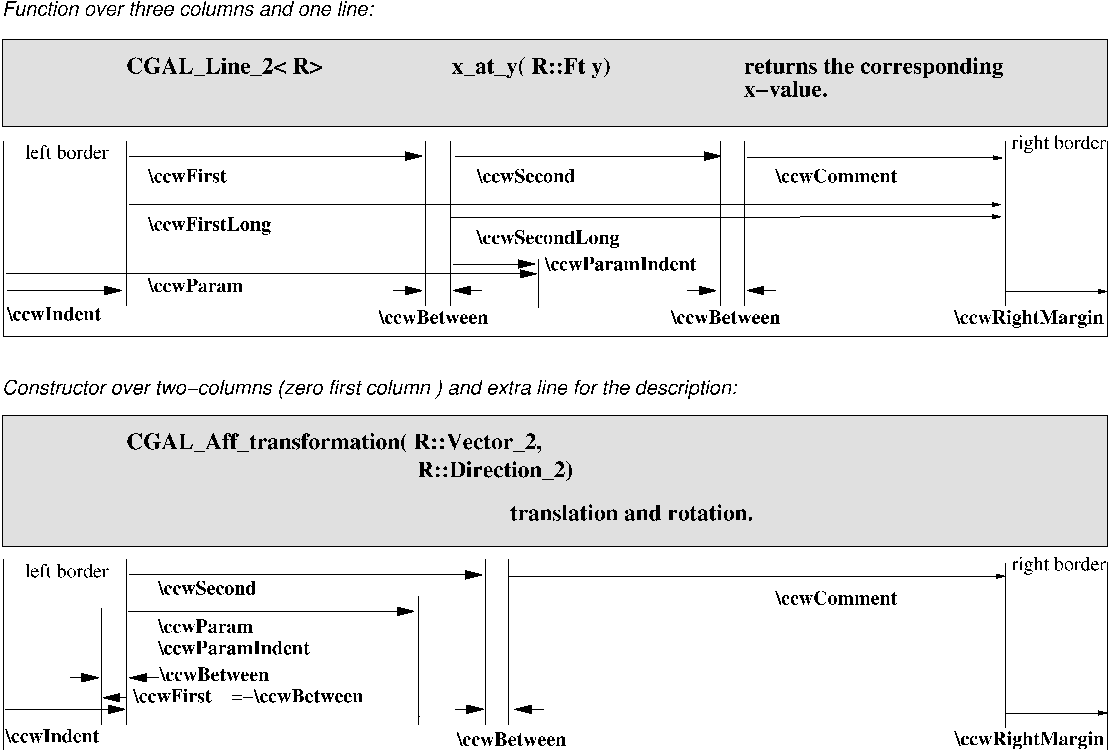
\includegraphics[width=1.0\textwidth]{Manual_tools/horizontal_struct}%
    \caption{Horizontal layout with two examples: A function that fits
      well in three columns and a constructor formatted in two
      columns and three lines.\index{horizontal layout}\index{layout}}}
    \label{figureHorizontal}\figuretopindent
\begin{ccHtmlOnly}
<CENTER>
   <IMG SRC="Manual_tools/horizontal_struct.gif" ALT="Horizontal layout with two examples: A function that fits well in three columns and a constructor formatted in two columns and three lines.">
</CENTER>
\end{ccHtmlOnly}
\end{figure}

\lcTex{\ccwIndent=7mm}
\ccSetTwoColumns{template <class T> struct A \{\};}{}
\ccStruct{template <class T> struct A {};}{in a separate line.}
\def\ccTagTemplateInline{\ccTrue}
\ccStruct{template <class T> struct A {};}{in a single line.}
\def\ccTagTemplateInline{\ccFalse}
\lcTex{\ccwIndent=0mm}

For the full reference, please take a look at the style itself, it is
quite well documented. A few more details to understand the style file
are given here. Two examples are given at the end of this section.
They demonstrate the use of the different dimensions to format own
pieces in the column layout.  The layout is mainly determined by the
dimensions found in the first section of the style file. They are named
with the prefix \verb+\ccw+. Several of them can be calculated
automatically from \verb+\ccwFirst+, \verb+\ccwSecond+,
\verb+\ccwIndent+, and \verb+\ccwRightMargin+ with the macro
\verb+\ccInitWidths+ which is called prior to each declaration
formatting.  The \Dindex{three-column layout} uses
\verb+\ccwFunctionFirst+ and \verb+\ccwFunctionSecond+ to set the
dimensions \verb+\ccwFirst+ and \verb+\ccwSecond+. This is
automatically done with the macro \verb+\ccInitFunctionWidths+.  The
two-column layout uses \verb+\ccwConstructorFirst+ and
\verb+\ccwConstructorSecond+. The appropriate initialization is the
macro \verb+\ccInitConstructorWidths+. Note that the
\verb+\ccwConstructorFirst+ is fixed to \verb+-1\ccwBetween+ which
compensates the padding space between the empty first column and the
second column.

Two pairs of commands are available that allow you to save and restore these
column width values easily when, for example, you want to change the
formatting for only a single function or class.  These commands
are:\verb|\ccSaveThreeColumns|%
\ccIndexEntry{SaveThreeColumns} and \verb|\ccRestoreThreeColumns|%
\ccIndexEntry{RestoreThreeColumns}, which save the current values of
\verb|\ccwFunctionFirst| and \verb|\ccwFunctionSecond| in temporary
variables and then restore them; and \verb|\ccSaveTwoColumns|%
\ccIndexEntry{SaveTwoColumns} and \verb|\ccRestoreTwoColumns|%
\ccIndexEntry{RestoreTwoColumns}, which save the current value of
\verb|\ccwConstructorSecond| and then restore it.

The other two dimensions, \verb+\ccwIndent+ and
\verb+\ccwRightMargin+, are useful to narrow the original
\verb+\textwidth+ for the declarations as in the following
example.

\lcTex{
\ccwIndent=7mm
\ccwRightMargin=10mm
}
\ccFunction{int foo(X x);}{A bit more text to demonstrate the right margin.}
\ccFunction{template<class A> int bar(A a);}{A bit more text to
  demonstrate the right margin.}
\lcTex{
\ccwIndent=0mm
\ccwRightMargin=0mm
}

A few macros for the vertical layout structuring follow in the style.
If multiple declarations should be formatted without any vertical
space in between, the macro \verb+\ccGlueDeclarations+ glues them
together (abbr.\ \verb+\ccGlue+).
Another possibility to get a more dense layout is to
redefine the \verb+\parskip+ parameter to zero. The original settings
for \verb+\parskip+ and \verb+\parindent+ can be restored using
\verb+\ccParDims+. The macro pair \verb+\ccGlueBegin+ and
\verb+\ccGlueEnd+ enclosing the set of declarations works a bit more
sophisticated.
\ccIndexEntry{GlueDeclarations}\ccIndexEntry{ParDims}\Mindex{parskip}\Mindex{parindent}
\ccIndexEntry{Glue}\ccIndexEntry{GlueBegin}\ccIndexEntry{GlueEnd}

\index{layout by hand}
Figure~\ref{figureHorizontal} and~\ref{figureVertical} show
sample layouts and the dimensions involved. The following example
demonstrates the use of the different dimensions to achieve a three
column layout using one line:

\begin{figure}
\lcTex{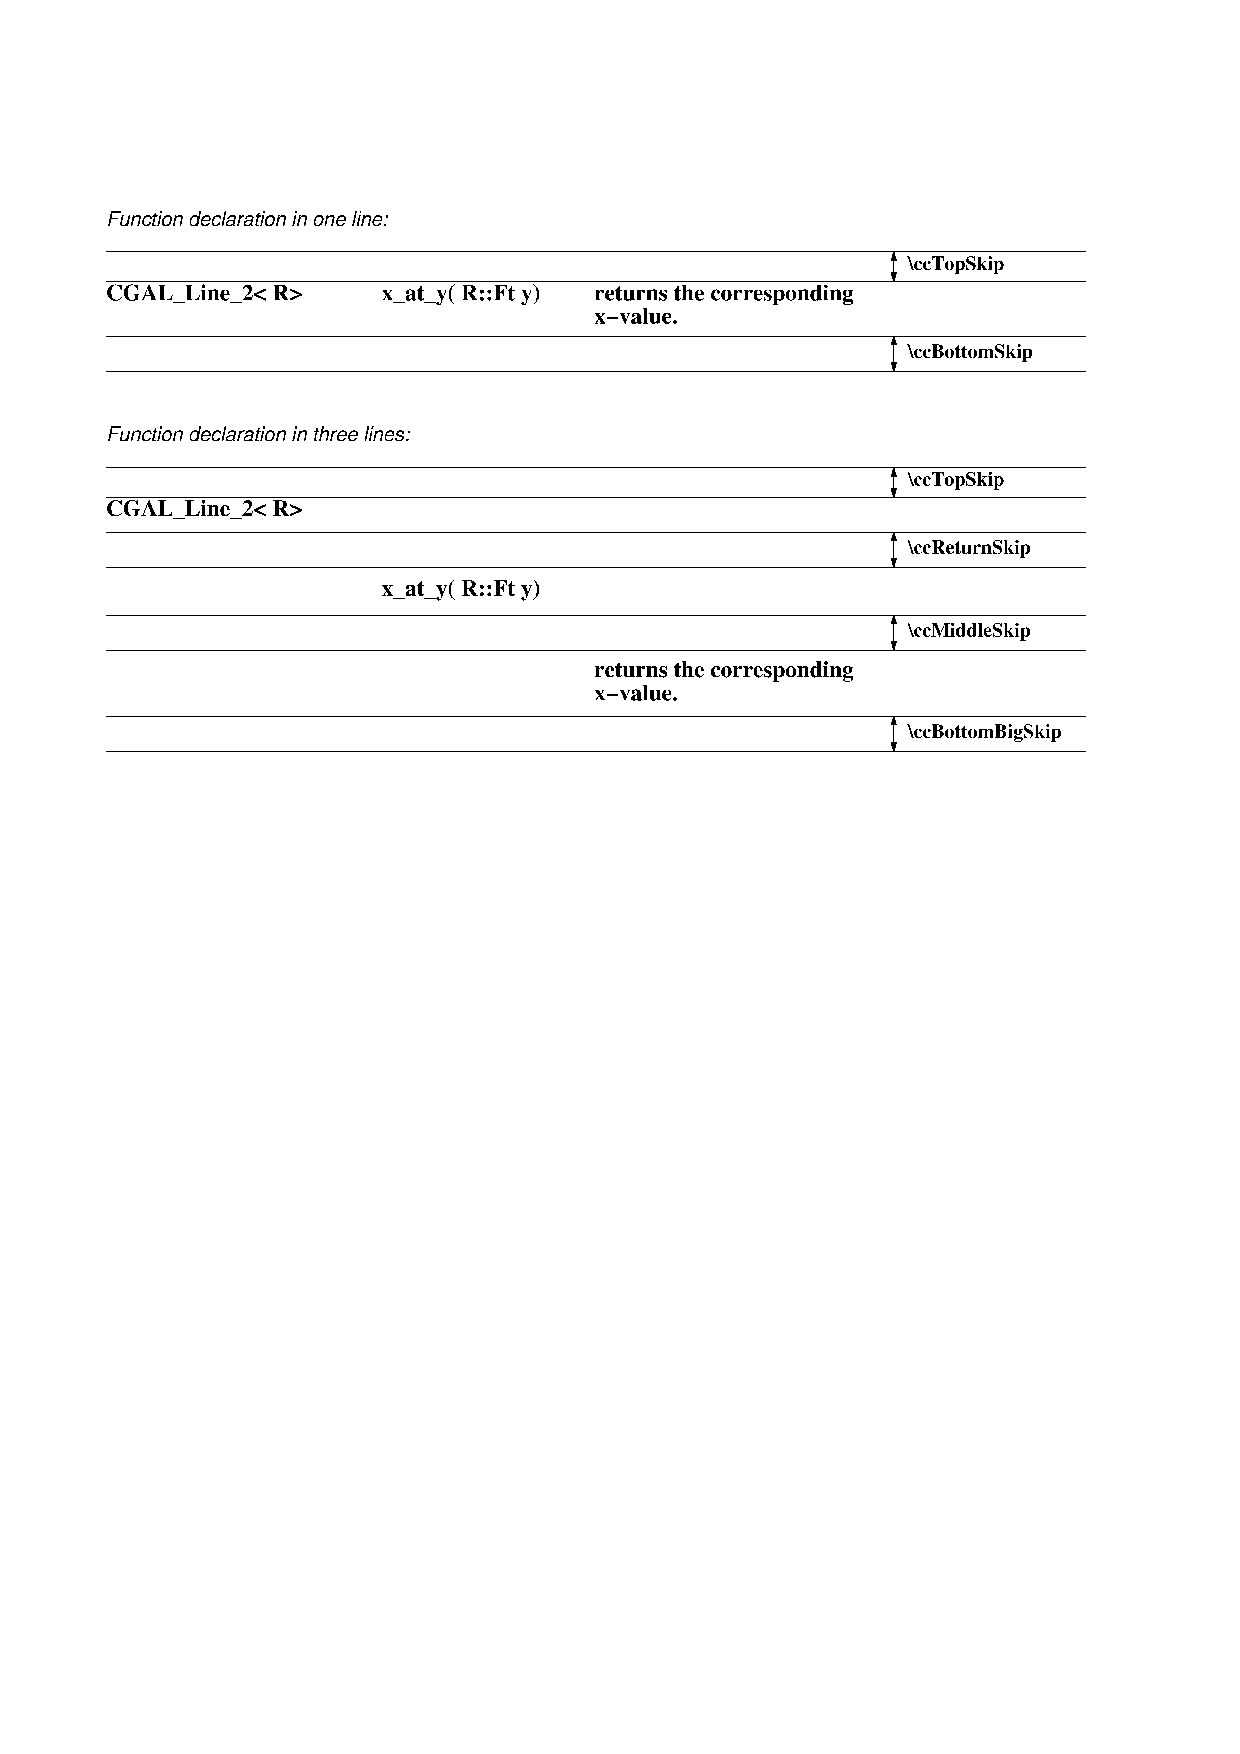
\includegraphics[width=1.0\textwidth]{Manual_tools/vertical_struct}%
    \caption{Vertical layout with two examples: A function that fits well
      in three columns, and a function
      formatted in three lines.\index{vertical layout}\index{layout}}}
    \label{figureVertical}\figuretopindent
\begin{ccHtmlOnly}
<CENTER>
  <IMG SRC="Manual_tools/vertical_struct.gif" ALT="Vertical layout with two examples: A function that fits well in three columns, and a function formatted in three lines.">
</CENTER>
\end{ccHtmlOnly}
\end{figure}

\begin{verbatim}
\ccSetThreeColumns{return-type}{function()}{}
\ccInitFunctionWidths
\ccTopSkip\hspace*{\ccwIndent}\parbox[t]{\ccwFirst}{%
    \ccStyle{return-type}%
}\hspace*{\ccwBetween}\parbox[t]{\ccwSecond}{%
    \ccStyle{function()}%
}\hspace*{\ccwBetween}\parbox[t]{\ccwComment}{%
    a comment. A bit more text is necessary to demonstrate that the
    comment formats nicely in the third column.
}\ccBottomSkip
\end{verbatim}

\ccSetThreeColumns{return-type}{function()}{}
\ccInitFunctionWidths
\ccTopSkip\hspace*{\ccwIndent}\parbox[t]{\ccwFirst}{%
    \ccStyle{return-type}%
}\hspace*{\ccwBetween}\parbox[t]{\ccwSecond}{%
    \ccStyle{function()}%
}\hspace*{\ccwBetween}\parbox[t]{\ccwComment}{%
    a comment. A bit more text is necessary to demonstrate that the
    comment formats nicely in the third column.
}\ccBottomSkip

Another example demonstrates the use of the different dimensions to
achieve a three-column layout where each column entry needs a new
line:

\begin{verbatim}
\ccTopSkip\hspace*{\ccwIndent}%
    \ccStyle{a-long-and-silly-return-type}%
\par\hspace*{\ccwIndent}\hspace*{\ccwFirst}\hspace*{\ccwBetween}%
    \ccStyle{function( int arg1, int arg2, int arg3, int arg4)}%
\par\hspace*{\ccwIndent}\hspace*{\ccwFirst}\hspace*{\ccwBetween}%
\hspace*{\ccwSecond}\hspace*{\ccwBetween}\parbox[t]{\ccwComment}{%
    a comment. A bit more text is necessary to demonstrate that the
    comment formats nicely in the third column.
}\ccBottomBigSkip
\end{verbatim}

\ccTopSkip\hspace*{\ccwIndent}%
    \ccStyle{a-long-and-silly-return-type}%
\par\hspace*{\ccwIndent}\hspace*{\ccwFirst}\hspace*{\ccwBetween}%
    \ccStyle{function( int arg1, int arg2, int arg3, int arg4)}%
\par\hspace*{\ccwIndent}\hspace*{\ccwFirst}\hspace*{\ccwBetween}%
\hspace*{\ccwSecond}\hspace*{\ccwBetween}\parbox[t]{\ccwComment}{%
    a comment. A bit more text is necessary to demonstrate that the
    comment formats nicely in the third column.
}\ccBottomBigSkip



% -------------------------------------------------
\subsection*{Rules for Simplifying \CC\ Declarations}
\label{sectionRulesSimple}
\index{reduction rules}
\index{simplification rules}

\CC\ declarations are simplified for more readability according to the
rules described in Section~\ref{sectionDeclarations}. These rules can
be activated or deactivated by setting the following tags to the
appropriate truth value \verb+\ccTrue+ or
\verb+\ccFalse+. By default they are all activated, i.e.\ set to
\verb+\ccTrue+. All rules can be deactivated at once with the
macro \verb+\ccTagFullDeclarations+ and restored to their default
value using the macro \verb+\ccTagDefaults+.
\ccIndexEntry{TagFullDeclarations}\ccIndexEntry{TagDefaults}\ccIndexEntry{True}\ccIndexEntry{False}

The first tag \verb+\ccTagRmConstRefPair+ controls whether {\tt
  const\ldots\&}-pairs are removed or not. The second tag
\verb+\ccTagRmEigenClassName+ controls whether the name of a
class within a class environment is removed from function argument
lists. The third tag \verb+\ccTagOperatorLayout+ controls
whether an operator declaration is formatted as a function declaration
or in operator notation. The fourth tag
\verb+\ccTagRmTrailingConst+ controls the appearance of the
part of a constructor or member function declaration after the closing
parenthesis. This is the {\tt const}-keyword if any. An example is
given using all simplifications rules and none. Note that this could
also be achieved with the macro \verb+\ccTagFullDeclarations+.
We assume that we are within a class environment for the class
\ccStyle{Gnat}.
\ccIndexEntry{TagRmConstRefPair}\ccIndexEntry{TagRmEigenClassName}
\ccIndexEntry{TagOperatorLayout}\ccIndexEntry{TagRmTrailingConst}

\begin{ccClass}{Gnat}
\lcTex{\ccwIndent7mm}
\ccSetThreeColumns{intM}{g.operator+( const Gnat& a) const;}{}
\ccCreationVariable{g}

\ccMethod{int operator+(const Gnat& a) const;}{all rules active.}
\vspace{-2ex}

\begin{tabbing}
\lcTex{ \hspace*{5.5mm} \= CCimplementationNNNMMMMMMMMMMMMMMMMMMMM \=
                   ImplementationMMMMM \= \kill }
  \> \verb+\def\ccTagRmConstRefPair{\ccFalse}+\\
  \> \verb+\def\ccTagRmEigenClassName{\ccFalse}+\\
  \> \verb+\def\ccTagOperatorLayout{\ccFalse}+\\
  \> \verb+\def\ccTagRmTrailingConst{\ccFalse}+
\end{tabbing}
\vspace{-2ex}

\ccTagFullDeclarations
\ccMethod{int operator+(const Gnat& a) const;}{all rules off.}

\ccIndexEntry{TagFullDeclarations}\ccIndexEntry{TagDefaults}\ccIndexEntry{True}\ccIndexEntry{False}
\begin{tabbing}
\lcTex{  \hspace*{5.5mm} \= CCimplementationNNNMMMMMMMMMMMMMMMMMMMM \=
                   ImplementationMMMMM \= \kill }
  \> \verb+\ccTagFullDeclarations+ \\
  \> \verb+\ccTagDefaults+
\end{tabbing}

\end{ccClass}
\ccTagDefaults

\index{empty parameter}\ccIndexEntry{ClassTemplateName}
In the unlikely but possible case that in a function argument list an
argument vanishes completely due to the reduction rules the
\verb+\ccClassTemplateName+ is shown.

Another rule that is switched off by default is the removal of the template
keyword including its argument list from template declarations. It is
controlled with the tag \verb+\ccTagRmTemplate+. It is set to
\verb+\ccFalse+ by \verb+\ccTagDefaults+ and also by
\verb+\ccTagFullDeclarations+.


% -------------------------------------------------
\subsection*{Formatting Style for \CC\ Code}
\index{formatting style}
\index{C++ formatting@\CC\ formatting}

The font and style in which the declarations are formatted can be
changed by overwriting the macros \verb"\ccFont" and \verb"\ccEndFont".
Their default settings are:
\ccIndexEntry{Font}\ccIndexEntry{EndFont}

\begin{tabbing}
\lcTex{  M \= CCimplementationNNNMMMMMMMMMMMMMMMMMMMM \= ImplementationMMMMM \= \kill}
  \> \verb+\newcommand{\ccFont}{\it}+ \\
  \> \verb+\newcommand{\ccEndFont}{\/}+
\end{tabbing}

They are used within a group, so font changing commands are local. A
typical usage is to change the style to \verb+\tt+-style as follows.
The example thereafter demonstrates the effect with a short function
declaration.

\begin{tabbing}
\lcTex{  M \= CCimplementationNNNMMMMMMMMMMMMMMMMMMMM \= ImplementationMMMMM \= \kill}
  \> \verb+\renewcommand{\ccFont}{\tt}+ \\
  \> \verb+\renewcommand{\ccEndFont}{}+
\end{tabbing}
\vspace{-\parskip}

\ccSetThreeColumns{intM}{foo(X x);M}{}
\lcTex{
\ccwIndent=6mm
\ccwRightMargin=10mm
}
\renewcommand{\ccFont}{\tt}\renewcommand{\ccEndFont}{}
\ccFunction{int foo(X x);}{a declaration formatted in teletypewrite.}
\renewcommand{\ccFont}{\it}\renewcommand{\ccEndFont}{\/}
\lcTex{
\ccwIndent=0mm
\ccwRightMargin=0mm
}

\index{font changes}\index{change font}
For special purposes the \Dindex{formatting style} can be changed within the
\CC\ declaration with the usual \LaTeX\ font changing macros. The
following example is generated with
\verb+\tt k-th\ccFont -dim \tt k-th\ccFont -foo;+ in the \CC\
declaration part of a \verb+\ccVariable+ macro. Please note that the
use of \LaTeX\ macros within the \CC\ declaration is {\em not} recommended,
because they are not supported by the other tools and their
interference with the programming in the style might be unpredictable,
e.g. the font can be changed for classnames too, but only if the
removal rule for the own classname in argument lists is switched of
(tag \verb+\ccTagRmEigenClassName+, Section~\ref{sectionRulesSimple}).
\ccIndexEntry{TagRmEigenClassName}

\lcTex{\ccwIndent=6mm}
\ccSetThreeColumns{\tt k-th\ccFont -dim}{\tt k-th\ccFont -foo;}{}
\ccVariable{\tt k-th\ccFont -dim \tt k-th\ccFont -foo;}{%
    a {\tt k-th}-dimensional variable.}
\lcTex{\ccwIndent=0mm}

A couple of \Dindex{special characters} are also changeable with a
\verb+\renewcommand+~:
\ccIndexEntry{Underscore}\ccIndexEntry{Hat}\ccIndexEntry{OpenAngle}
\ccIndexEntry{Ampersand}\ccIndexEntry{CloseAngle}\ccIndexEntry{Tilde}

\begin{tabbing}
\lcTex{
  M \= +foo ccUnderscore bar M \= foo\ccUnderscore barMMM
    \= +foo ccAmpersand bar M \= foo\ccAmpersand bar\kill }

  \> \verb+foo\ccUnderscore bar+      \> {\em foo\ccUnderscore bar} \>
     \verb+foo\ccHat bar+             \> {\em foo\ccHat bar} \\
  \> \verb+foo\ccOpenAngle bar+       \> {\em foo\ccOpenAngle bar} \>
     \verb+foo\ccAmpersand bar+       \> {\em foo\ccAmpersand bar} \\
  \> \verb+foo\ccCloseAngle bar+      \> {\em foo\ccCloseAngle bar} \>
     \verb+foo\ccTilde bar+           \> {\em foo\ccTilde bar}
\end{tabbing}

% -------------------------------------------------
\subsection*{Replacement of a Name Prefix}
\index{name prefix replacement}
\index{replacement, name prefix}
\index{prefix|see{name prefix}}

\ccIndexEntry{SrcPrefix}\ccIndexEntry{TargetPrefix}\ccIndexEntry{TagReplacePrefix}
\ccIndexEntry{TagReplaceInclude}\ccIndexEntry{True}\ccIndexEntry{False}
\ccIndexEntry{TagDefaults}\ccIndexEntry{Style}\TTindex{cprog.sty}

\index{name prefix}
The external identifiers in \cgal\ were originally prefixed with {\tt CGAL\_}
before the conversion to the \cgal\ namespace. The {\tt cc\_manual.sty}
therefore offers two possibilities to change this prefix: The prefix is removed
or the prefix is changed to another prefix. In the latter case the
prefix {\tt CGAL/} for the include files of the library is probably
also a subject of change. Before activating the prefix substitution
the macros \verb+\ccSrcPrefix+ and \verb+\ccTargetPrefix+ have to be
set with the \TeX\ \verb+\def+ or \verb+\gdef+ macros. The special character
{\tt \_} or {\tt /} must not be part of these prefixes here. Both are
set to {\tt CGAL} by default. To activate the substitution for the
identifier prefix with the {\tt \_} set the tag
\verb+\ccTagReplacePrefix+ to \verb+\ccTrue+. To activate additionally
the substitution for the file name paths set the tag
\verb+\ccTagReplaceInclude+ to \verb+\ccTrue+. Both tags will be
reset with the macro \verb+\ccTagDefaults+. The replacing code will
work on merely all \CC\ code that is placed within the declaration
macros or the macro \verb+\ccStyle+. However, macros from other
packages are not influenced, e.g., example programs formatted within
the \verb+\cprog+ or \verb+\verbatim+ environments.

The example illustrates both typical usages (with a fantasy function
that does not exist in \cgal).

\lcTex{\ccwIndent=6mm}
\ccSetThreeColumns{CGAL_Point<R>}{CGAL_f( CGAL_Vector<R> v)}{}

\hspace*{6mm}\ccStyle{#include <CGAL/Point_2.h>}
\\
\ccFunction{CGAL_Point<R> CGAL_f( CGAL_Vector<R> v);}{%
    the original \cgal\ prefix.}
\vspace{-\parskip}

\begin{tabbing}
\lcTex{  M \= CCimplementationNNNMMMMMMMMMMMMMMMMMMMM \= ImplementationMMMMM \= \kill}
  \> \verb+\def\ccTargetPrefix{}+ \\
  \> \verb+\def\ccTagReplacePrefix{\ccTrue}+
\end{tabbing}
\def\ccTargetPrefix{}
\def\ccTagReplacePrefix{\ccTrue}
\vspace{-\parskip}

\hspace*{6mm}\ccStyle{#include <CGAL/Point_2.h>}
\\
\ccFunction{CGAL_Point<R> CGAL_f( CGAL_Vector<R> v);}{%
    assuming name spaces. {\tt ;-)}}
\vspace{-\parskip}

\begin{tabbing}
\lcTex{  M \= CCimplementationNNNMMMMMMMMMMMMMMMMMMMM \= ImplementationMMMMM \= \kill}
  \> \verb+\def\ccTargetPrefix{GTE}+ \\
  \> \verb+\def\ccTagReplaceInclude{\ccTrue}+
\end{tabbing}
\def\ccTargetPrefix{GTE}
\def\ccTagReplaceInclude{\ccTrue}
\vspace{-\parskip}

\hspace*{6mm}\ccStyle{#include <CGAL/Point_2.h>}
\\
\ccFunction{CGAL_Point<R> CGAL_f( CGAL_Vector<R> v);}{%
    transform it to a Porsche.}
\vspace{-\parskip}

\begin{tabbing}
\lcTex{  M \= CCimplementationNNNMMMMMMMMMMMMMMMMMMMM \= ImplementationMMMMM \= \kill}
  \> \verb+\def\ccTagReplacePrefix{\ccFalse}+ \\
  \> \verb+\def\ccTagReplaceInclude{\ccFalse}+
\end{tabbing}
\def\ccTagReplacePrefix{\ccFalse}
\def\ccTagReplaceInclude{\ccFalse}

\lcTex{
\ccwIndent=0mm
\ccwRightMargin=0mm
}


% -------------------------------------------------
\subsection*{Miscellaneous Options}
\label{sectionCustomizeMisc}
\index{miscellaneous customization options}

\ccIndexEntry{Hidden}\ccIndexEntry{Declaration}\ccIndexEntry{MakeAllVisible}
The macros \verb+\ccHidden+ and \verb+\ccDeclaration+ from
Section~\ref{sectionDeclarations} allow the writing of \CC\
declarations that are only visible for the checking program and not in
the manual. This can be changed using the macro \verb+\ccMakeAllVisible+.
It redefines both macros to format their parameters also in the
manual. The effect cannot be reversed. For the macro
\verb+\ccDeclaration+ the macro \verb+\ccStyle+ is used for the
formatting. The \verb+\ccHidden+ macro vanishes simply exposing the
declaration thereafter.


\ccIndexEntry{ChapterAuthor}\ccIndexEntry{TagChapterAuthor}
\ccIndexEntry{ChapterRelease}\ccIndexEntry{TagChapterRelease}
\ccIndexEntry{False}\ccIndexEntry{True}\ccIndexEntry{TagDefaults}

The macros \verb+\ccChapterAuthor+ and \verb+\ccChapterRelease+ from
Section~\ref{sectionStructureMacros} format their parameters as
authors or release number of a chapter.  The author macro is switched
on and the release macro is switched off by default. These settings
can be changed by setting the tags \verb+\ccTagChapterAuthor+ and
\verb+\ccTagChapterRelease+ to \verb+\ccFalse+ or \verb+\ccTrue+,
respectively. The macro \verb+\ccTagDefaults+ resets them to their
defaults.

% ----------------------------------------------------------------------
\section{Revision History and Changes}
\label{sectionChanges}
\index{revision history}\index{changes}
\index{revision notes}


\begin{description}
 % ----------------------------------------------------
    \item[Revision: 3.12~~~Date: 2002/08/23]~\\[-3mm]
    \begin{itemize}
       \item New macros \verb|\ccRefChapter| and \verb|\ccUserChapter| introduced.
          \end{itemize}
    % ----------------------------------------------------
    \item[Revision: 3.11~~~Date: 2001/08/20]~\\[-3mm]
    \begin{itemize}
       \item added \verb|\ccRefPageNumAtMargin| that allows you to change the
             appearance of page numbers produced by the commands.
             \verb|\ccRefIdfierPage| and \verb|\ccRefConceptPage|.
             If this is set to true (default), the page numbers appear at the
             right margin with the space in between filled using
             \verb+\ccRefPageFill+.  When false, the page numbers appear
             directly after the name using the following format ``(pg. \#)''.
       \item added command \verb|\ccRefPageBreak| that can be used to turn off
             and on page breaks that occur at the beginning and end of each
             \verb|\ccRef*| section.
       \item added \verb|\ccRequire| and \verb|\ccRequirements| commands.
             The first is like \verb|\ccPrecond| and generates a comment
             heading with text ``Requirement''. The second generates a
             boldface heading like \verb|\ccDefinition| with the text
             ``Requirements''.
       \item added command \verb|\listofrefpages|, analogous to the
             \verb|\listoffigures| command, which produces a listing of
             all refernece pages in the PostScript manual.  The listing
             can be made alphabetical using the Unix \verb|sort| command.
       \item added commands \verb|\ccMultiplePartsToc| and
             \verb|\ccNumberChaptersByPart|
             to allow manuals with separate parts.  The first tells the
             HTML converter that its table of contents should be formatted
             properly for a manual with multiple parts and the second
             tells both HTML and \LaTeX to start numbering chapters at
             1 with each new part.
    \end{itemize}
    % ----------------------------------------------------
    \item[Revision: 3.10~~~Date: 2001/04/02]~\\[-3mm]
    \begin{itemize}
       \item added the command \verb|\ccRefines| that creates a new
             heading for a class
       \item added the commands \verb|\ccHtmlNoRefLinks|
             and \verb|\ccHtmlNoRefIndex| that turn off, respectively,
             linking and indexing of reference page identifiers.
       \item added command \verb|\ccRefPageFill|, which is the command used
             by \verb|\ccRefIdfierPage| and \verb|\ccRefConceptPage| to fill
             the space between a reference page identifier name and
             the page number (default is \verb|\dotfill|).
       \item fixed bug in HTML converter that duplicated the local scopes
             given in the headings of reference pages in the prefixes of
             nested types, {\em etc.}
       \item fixed bug that caused operators to disappear in the
             PostScript manual when \verb|ccTagOperatorLayout| was set to false.
    \end{itemize}
    % ----------------------------------------------------
    \item[Revision: 3.9~~~Date: 2000/09/01]~\\[-3mm]
    \begin{itemize}
       \item added commands \verb|\ccHtmlLinksOff|, \verb|\ccHtmlLinksOn|,
             and \verb|\ccHtmlNoLinksFrom| that allow one to cause links not
             to be created in the HTML manual for the text delimited by
             these commands.
    \end{itemize}
    % ----------------------------------------------------
    \item[Revision: 3.8~~~Date: 2000/08/02]~\\[-3mm]
    \begin{itemize}
        \item Fixed bug in \verb|\ccRefConceptPage| for HTML conversion
        \item Fixed bug in HTML converter that did not attach the local scope
              to reference page labels, files, {\em etc.}
        \item Fixed HTML converter so it does not generate file names
              containing $<$, $>$ or $:$ (which Microsoft doesn't like).
    \end{itemize}
    % ----------------------------------------------------
    \item[Revision: 3.7~~~Date: 2000/07/31]~\\[-3mm]
    \begin{itemize}
        \item Fixed bugs in {\tt cc\_manual\_index.sty} causing problems with
              modified items and concepts as subitems.
        \item Fixed bug in {\tt ccInclude} macro in {\tt latex\_converter.sty}
              that caused the item following such a command not to be linked
              when include files were not linked.
        \item Changed the tabs for the new manual style so they are now in
              color.
        \item Changed {\tt ccAdvanced} envrionment brackets to include the
              word "advanced".
        \item Added environments {\tt ccRefConstant},
              {\tt ccRefFunctionObjectConcept}, and
              {\tt ccRefFunctionObjectClass}.
        \item Added heading commands \verb|\ccGeneralizes| and
              \verb|\ccQueryFunctions|.
        \item Added \verb|\ccRefConceptPage| command to be used instead of
              \verb|\ccRefIdfierPage| for concepts so the font for the concepts
              is correct.
        \item Added commands \verb|\ccSaveThreeColmns|,
              \verb|\ccRestoreThreeColumns|, \verb|\ccSaveTwoColumns|,
              and \verb|\ccRestoreTwoColumns| that save and restore column
              widths for help in temporarily changing formatting.
    \end{itemize}
    % ----------------------------------------------------
    \item[Revision: 3.6~~~Date: 2000/05/17]~\\[-3mm]
    \begin{itemize}
       \item  Modified \verb|cc_extract_html| so it now uses the environment
              variable \verb|LATEX_CONV_INPUTS| to search for input files.
              This is analogous to the \verb|TEXINPUTS| environment variable
              used by \LaTeX.  If
              \verb|LATEX_CONV_INPUTS| is set, files are searched for in the
              indicated directories in the indicated order; if not set, files
              are searched for in the current directory.
       \item  Modified the indexing and fromatting commands for \LaTeX, so
              now underscores are allowed in concept names but no other
              ``special'' characters.  Concept names are displayed in the
              default font in both the body and the index. (Note: This
              is true only for the PostScript manual; in the HTML manual,
              concept names are still displayed in italics.)
       \item  Changed test suite and {\tt cc\_check} script so they do
              not assume the current directory is in your path.
       \item  Fixed a bug in \verb|cc_manual.sty| that was placing the global
              scope string ({\em e.g.} ``CGAL::'') before concept names in page
              headers.
       \item  Fixed a bug in \verb|cc_manual_index.sty| for index entries
              produced by the \verb|\ccRef...| environments that were not
              formatted using \verb|\ccFont| when the optional scope argument
              was used.
       \item  Made \verb|cc_manual.sty| include the package \verb|graphicx| if
              the new manual style is used, since this is where the
              \verb|\includegraphics| command that is used to include the side
              tabs for the reference pages is defined.
       \item  Made \verb|cc_manual_index.sty| include the \verb|makeindex|
              package.
       \item  Added the do-nothing command \verb|\printindex| to
              the HTML version of \verb|latex.sty|.
       \item  Added a \verb|\cc_manual_index.sty| file to the HTML style files.
              This simply defines all the indexing commands that might appear
              in the text, but they currently do nothing.
    \end{itemize}


    % ----------------------------------------------------
    \item[Revision: 3.5~~~Date: 2000/01/27]~\\[3mm]
    %
    The following bugs and problems are remedied with this release:
    \begin{itemize}
       \item In the \verb|\parseText| macro of \verb|cc_manual_index.sty| the
             variable \verb|\text| was renamed to \verb|\indexText| to avoid
             a conflict with the existing AMS-\LaTeX\ \verb|\text| command.
       \item In \verb|cc_extract_html| (in \verb|cpp_formatting.C|), fixed a
             formatting problem that left off the template parameters from
             nested types and typedefs in the HTML index.
       \item Added missing command \verb|\galia| to HTML \verb|cc_manual.sty|
             file.
       \item Added a new style file {\tt nonlinkedpath.sty} in the release.
             This file defines the command \verb|\nonlinkedpath|, which
             behaves the same as the \verb|\path| command, except it
             does not create a link in the HTML manual.
       \item Modified {\tt cc\_manual.sty} to include the
             {\tt cc\_manual\_index.sty} and {\tt alltt.sty} style files upon
             which it depends.  Similarly modified {\tt cc\_manual\_index.sty}
             to include {\tt cc\_manual.sty} since it uses commands defined
             there.
       \item Fixed a problem with the figure and table environments for
             the {\tt latex.sty} file that caused problems when optional
             arguments indicating placement preferences were used.
       \item Changed the names of the HTML files created to remove the
             special characters (such as \verb|<| and \verb|>|) that are
             not supported under Microsoft windows.
       \item Updated the documentation of {\tt cc\_manual.sty} and
             {\tt cc\_manual\_index.sty} to include
             appendices that summarize all commands and to fix a few
             inconsistencies with the style files.
    \end{itemize}

    % ----------------------------------------------------
    \item[Revision: 3.4~~~Date: 1999/09/27]~\\[3mm]
    %
    Added new \LaTeX\ style file \verb|cc_manual_index.sty| that contains
    macros for producing an index for the PostScript version of the manual.
    This style file is documented separately.
    The style file \verb|cc_manual.sty| has been modified to allow for
    automatic indexing of most of the \CC\ names that are formatted with the
    macros in this style file.

    % ----------------------------------------------------
    \item[Revision: 3.3~~~Date: 1999/09/07]~\\[3mm]
    %
    Updated documentation and a new example directory showing the new
    style of reference manual pages. The documentation is split into
    three manuals. The documentation could still be enhanced for the
    \LaTeX\ to HTML converter. A few bug fixes and some heavy cleanups
    are done in the source code and other distributed files. The old
    slides are no longer distributed. Maintenance for \cgal\ is taken
    over by Susan Hert.

    % ----------------------------------------------------
    \item[Revision: 3.2~~~Date: 1999/08/24]~\\[3mm]
    %
    HTML converter and \verb+cc_manual.sty+ support the new manual
    reference manual style (incl.~tabs at the side margins) and
    the style for the intermediate transition period. Several bugs
    have been fixed. The documentation lacks all the new features
    and will be updated for the next release.

    % ----------------------------------------------------
    \item[Revision: 3.1~~~Date: 1998/08/05]~\\[3mm]
    %
    Major rewrite of the HTML converter. New features: Full support of
    \LaTeX\ macro definitions with newcommand/newenvironment/newtheorem
    including parameters and a mechanism for optional parameter support.
    Support for \TeX-style macro definitions, except where pattern
    matching is used. Better support for math symbols. All symbols listed
    in the Leslie Lamport book are available. If not directly supported in
    HTML, they are included as inline GIF images. In addition
    \verb+\mathcal+ and \verb+\mathbb+ are supported with uppercase letters.
    Font style changes are fully supported including font size changes and
    small caps font shape (small caps may produce unpredictable results
    if other non-trivial macros are used within a small caps text).
    Only limited table and formula support. No figure or PostScript
    picture support.

    Further extensions of the converter can be provided with style files,
    quite similar to \LaTeX-style files.

    The installation procedure has changed in favor of a single Makefile and
    support of environment variables, which allows the installation of future
    releases without configuring the Makefile and several scripts again and
    again.


    % ----------------------------------------------------
    \item[Revision: 2.16~~~Date: 1998/07/24]~\\[3mm]
    %
    Major rewrite of the HTML converter. This is the beta release of the
    upcoming 3.1 \LaTeX\ converter.

    % ----------------------------------------------------
    \item[Revision: 2.15~~~Date: 1998/04/08]~\\[3mm]
    %
    Removal of own class name fixed, such that it gets not removed
    if it is only a part of a larger idfier.

    % ----------------------------------------------------
    \item[Revision: 2.14~~~Date: 1998/04/01]~\\[3mm]
    %
    New macro \verb+\ccHtmlNoClassToc+ introduced.

    % ----------------------------------------------------
    \item[Revision: 2.13~~~Date: 1998/03/19]~\\[3mm]
    %
    Bug in {\tt cc\_manual.sty} with template declarations fixed.
    Parentheses removed from bibliography keys for HTML conversion.

    % ----------------------------------------------------
    \item[Revision: 2.12~~~Date: 1998/03/06]~\\[3mm]
    %
    Minor extensions and modifications: New macro \verb+\ccIncludeVerbatim+.
    The \TeX\ capacity error has been removed in the context of certain
    template function declarations.  HTML conversion enhanced, for example
    $\sqrt[k]{n}$ converts to something like root$_k(n)$. Wider format in HTML.

    % ----------------------------------------------------
    \item[Revision: 2.11a~~~Date: 1998/02/05]~\\[3mm]
    %
    Bug fix for the HTML converter. New release 2.12 of {\tt
    cc\_extract\_html}.

    % ----------------------------------------------------
    \item[Revision: 2.11~~~Date: 1997/12/19]~\\[3mm]
    %
    Minor extensions and modifications. New subsection \verb+\ccSeeAlso+.

    % ----------------------------------------------------
    \item[Revision: 2.10~~~Date: 1997/09/13]~\\[3mm]
    %
    The LEDA page dimension settings has been commented out. They were
    responsible for the faulty behavior of the \verb+\begin{verbatim}+
    environment where the space had no longer fixed size. The
    \ccc{operator()} and the type conversion operator are now correctly
    formatted when using \verb+\ccTagFullDeclarations+.  A \verb+\label+
    was automatically defined by the \verb+\ccSection+ macro. This has
    been removed. The new \verb+\ccChapterRelease+ macro with the
    corresponding \verb+\ccTagChapterRelease+ flag works like
    \verb+\ccChapterAuthor+. Both are switched off by default now.
    \verb+\ccNestedClass+ can be used in the global scope.

    Better configuration options are provided for the HTML conversion.
    The macros \verb+\ccHtmlNoLinks+ and \verb+\ccHtmlNoClassLinks+
    suppress the automatic generation of index entries.


    % ----------------------------------------------------
    \item[Revision: 2.9~~~Date: 1997/06/19]~\\[3mm]
    %
    A macro \verb+\stl+ for \stl\ has been added. A bug fix for the
    footnote placement in the HTML converter. It could have happened that
    footnotes appeared in wrong files and that the hyper-links to them
    failed.

    % ----------------------------------------------------
    \item[Revision: 2.8~~~Date: 1997/05/27]~\\[3mm]
    %
    The \verb+\ccEmptyParameter+ has been replaced by the
    \verb+\ccClassTemplateName+ in cases where necessary. Small extensions
    and a couple of bug fixes for the HTML support, including:
    \verb+\ref{}+ handling more robust. \verb+\ccc{}+ in math mode
    allowed. \verb+\ccHtmlNoClassIndex+ also inhibits member declarations
    from writing index entries. Single letter classes are no longer
    automatically cross linked. Math spacing like \verb+\;+ works again. Line
    numbers in error messages corrected.

    % ----------------------------------------------------
    \item[Revision: 2.7~~~Date: 1997/05/08]~\\[3mm]
    %
    Major extensions for the {\tt HTML} support. The mechanisms around the
    class environments are more flexible and can be used separately (file
    creation, indexing, cross linking), see
    Section~\ref{sectionHTMLsupport}. The {\tt HTML} converter supports
    now an additional file model for the manual with multiple
    subdirectories to avoid name clashes of class filenames and the cross
    referencing, see~\cite{k-lhcll-99}. The support for
    the automatic bibliography generation uses now the {\tt *.aux} file
    from \LaTeX\ to get the proper labels for the citation tags. The
    \verb+ccInclude+ macro converts to an anchor pointing to the actual
    header file. The \LaTeX\ style file {\tt path.sty} is supported
    with the \verb+\path+ macro to format URL's.


    % ----------------------------------------------------
    \item[Revision: 2.5~~~Date: 1997/04/24]~\\[3mm]
    %
    Bug fix for {\tt cc\_manual.sty}. The \verb+ccHtmlOnly+ environment
    failed. The \verb+\ccPrecond+ and \verb+\ccPostcond+ macros
    sometimes did not format in a separate line as they should. Long class
    names caused the \verb+\ccNestedClass+ macro to forget the type name.

    New section titles to structure a manual page. A new \verb+\ccInclude+
    macro and a script \verb+cc_extract_include+ extracting it. An
    environment \verb+ccAdvanced+ to mark paragraphs of advanced material.
    New method to glue multiple declarations together with
    \verb+\ccGlueBegin+ and \verb+\ccGlueEnd+.


    % ----------------------------------------------------
    \item[Revision: 2.4~~~Date: 1997/03/25]~\\[3mm]
    %
    Bug fix for {\tt cc\_manual.sty}. The keyword \verb+\end+ from \LaTeX\
    environments might have caused trouble with the {\tt cc\_manual.sty}
    internal parsing technique. Operators were not able to format argument
    lists with extra parentheses like for function pointer types.

    A few new abbreviations for often used macros: \verb+\ccc+
    for \verb+\ccStyle+, \verb+\ccThree+ for \verb+\ccSetThreeColumns+,
    \verb+\ccTwo+ for \verb+\ccSetTwoColumns+, \verb+\ccThreeToTwo+ for
    \verb+\ccPropagateThreeToTwoColumns+, and \verb+\ccGlue+ for
    \verb+\ccGlueDeclarations+.


    % ----------------------------------------------------
    \item[Revision: 2.3~~~Date: 1997/02/19]~\\[3mm]
    %
    Bug fix for {\tt cc\_manual.sty}. The removal of the class name in
    function argument lists failed with template classes (the template
    argument remained).  Member template constructors had not worked. No
    new manual release.

    % ----------------------------------------------------
    \item[Revision: 2.2~~~Date: 1997/02/16]~\\[3mm]
    %
    The default has changed that the style is no longer compatible with
    the revision 1.14. This can be  easily changed back. In the style file
    \verb+cc_manual.sty+ is a  macro \verb+\ccPortability+ in the first
    lines. It must be set to the value \verb+\ccTrue+ to activate the old
    names again. However, the supporting tools cannot support the old
    names. See below for scripts to help in renaming old
    files.\ccIndexEntry{Portability}

    The style has been extended with the \verb+\ccChapterSubTitle+ and
    \verb+\RCSdefDate+ macro. The handling of template declarations is
    made more flexible with the \verb+\ccTagTemplateInline+ and
    \verb+\ccTagRmTemplate+ tags. Small changes in the layout were made.

    The tools have been purified. A bug in the dynamic memory management
    of \verb+cc_extract+ and \verb+cc_build_checker+ has been removed. The
    {\tt cc\_manual\_to\_html} script uses now the {\tt CC} environment
    variable for the C compiler.

    The \verb+cc_manual_to_html+ converter handles now user defined macros
    (without parameters) and footnotes.

    % ----------------------------------------------------
    \item[Revision: 2.1~~~Date: 1997/01/22]~\\[3mm]
    %
    Major new release. If you still have to upgrade old documentations
    from revision 1.14 based on {\tt cgal\_manual.sty}, a \Dindex{Perl
    script}\index{scripts, Perl} helps in upgrading:
    {\tt cc\_update\_2.1} renames all of the older
    macros.\index{renaming macros}
\end{description}

% =====================================================
\newpage
\bibliographystyle{plain}
\bibliography{Manual_tools/manual}

\lcTex{\small
\printindex}

\appendix
\section{Quick Reference Guide}
\newcommand{\Indent}{\hspace*{5pt}}

In this appendix we summarize the various commands that are defined in
{\tt cc\_manual.sty} and provide either an example of the result or a
brief explanation of what the command does.  

\tablehead{
\hline
&  \\
{\large \bf Command} & {\large \bf Example and/or Result} \\ 
& \\ \hline \hline
}
\tabletail{\hline}

\begin{ccClassTemplate}{Gnu<T>}
\ccCreationVariable{g}
\begin{supertabular}{|p{7.4cm}|p{7.4cm}|} 

\verb|\CC| & \CC \Mindex{CC}\\ \hline

\verb|\ccAccessFunctions| 
&  \ccAccessFunctions 
\ccIndexEntry{AccessFunctions}\\ \hline 

& \\
\begin{minipage}{2.0in}
\verb|\begin{ccAdvanced}| \\
\VarText{text} \\
\verb|\end{ccAdvanced}|
\end{minipage} &
\begin{minipage}{3.0in}
\begin{ccAdvanced} 
\VarText{text}
\end{ccAdvanced} 
\end{minipage} 
\Eindex{ccAdvanced} \\ 
& \\ \hline

\verb|\ccAmpersand| 
& \leavevmode\ccAmpersand 
\ccIndexEntry{Ampersand}\\ \hline

\verb|\ccc{|\VarText{text}\verb|}|
&\verb+\ccc{A f_bar(X<T>& x = "%^~#");}+ \\
& \\
&\ccc{A f_bar(X<T>& x = "%^~#");} 
\ccIndexEntry{c}\\ \hline

&\verb|\def\ccTagChapaterAuthor{\ccTrue}| \\
\verb|\ccChapterAuthor{|\VarText{author name}\verb|}| 
&\verb|\ccChapterAuthor{Irene}| \\
& \\
&{\em Irene}  
\ccIndexEntry{ChapterAuthor}\\ \hline

&\verb|\def\ccTagChapterRelease{\ccTrue}| \\
\verb|\ccChapterRelease{|\VarText{release info}\verb|}|
&\verb|\ccChapterRelease{3.4, 4 February 2000}| \\
& \\
&{\em 3.4, 4 February 2000} 
\ccIndexEntry{ChapterRelease}\\ \hline

\verb|\ccChapterSubTitle{|\VarText{subtitle}\verb|}| 
&\verb|\ccChapterSubTitle{subtitle}| \\
& \\
&{\em subtitle} 
\ccIndexEntry{ChapterSubTitle} \\ \hline

\verb|\begin{ccClass}{|\VarText{class\_name}\verb|}| 
&\Indent \verb|\begin{ccClass}{My_class}| ...  \\
             \VarText{class description} 
& sets the variable \verb|\ccClassName| to \ccc{My_class} (formatted using \verb|\ccc|);  sets \verb|\ccPureClassName| to \verb|My_class| (without formatting) \\
        \verb|\end{ccClass}| 
&
\Eindex{ccClass} \\ \hline

\verb|\ccClassName| & 
the name of the current (nontemplated) class formated using
\verb|\ccc|
\ccIndexEntry{ClassName}  \\ \hline


\verb|\begin{ccClassTemplate}{|\VarText{class\_name}\verb|}| 
& \verb|\begin{ccClassTemplate}{Gnu<T>}| ...\\
    \VarText{class description} 
& sets variable \verb|\ccClassTemplateName| to \ccc{Gnu<T>}
(with template parameters) (formatted using \verb|\ccc|);
sets \verb|\ccPureClassTemplateName| to \verb|Gnu<T>| (without formatting) \\
\verb|\end{ccClassTemplate}| & 
\Eindex{ccClassTemplate} \\ \hline

\verb|\ccCloseAngle| & \leavevmode\ccCloseAngle
\ccIndexEntry{CloseAngle} \\ \hline

\verb|\ccCommentHeading{|\VarText{text}\verb|}| 
&\verb|\ccCommentHeading{comment heading}| \\
& \\
&\ccCommentHeading{comment heading}
\ccIndexEntry{CommentHeading} \\ \hline

\verb|\ccClassTemplateName| & 
the name of the current class with its template parameters
formated using \verb|\ccc|
\ccIndexEntry{ClassTemplateName}  \\ \hline

\verb|\ccConstants| & \ccConstants 
\ccIndexEntry{Constants} \\ \hline

\verb|\ccConstructor{|\VarText{header}\verb|}{|\VarText{comment}\verb|}| 
& \verb|\ccConstructor{Gnu(Gnu<T> a);}{comment}| \\
& \\
& \ccConstructor{Gnu(Gnu<T> a);}{comment}
\ccIndexEntry{Constructor} \\ \hline

\verb|\ccCreation| & \ccCreation 
\ccIndexEntry{Creation} \\ \hline

\verb|\ccCreationVariable{|\VarText{var\_name}\verb|}| & defines \VarText{var\_name} as the variable to use when formatting member functions for a class 
\ccIndexEntry{CreationVariable} \\ \hline

\verb|\ccDate| & prints the date of the {\tt cc\_manual.sty} file being used
\ccIndexEntry{Date} \\ \hline

\verb|\ccDeclaration{|\VarText{decl}\verb|}| 
& \VarText{decl} produces no text in the manual unless \verb|\ccMakeAllVisible| 
has been used; used only for the {\tt cc\_check} tool
\ccIndexEntry{Declaration} \\ \hline

\verb|\ccDefGlobalScope{|\VarText{scope\_name}\verb|}| & 
makes \VarText{scope\_name} the text that is prepended to all reference page 
names (except concepts)  (default: empty)
\ccIndexEntry{DefGlobalScope} \\ \hline

\verb|\ccDefinition| & \ccDefinition 
\ccIndexEntry{Definition} \\ \hline

\verb|\renewcommand{\ccEndFont}{|\VarText{chars}\verb|}| 
& \verb|\renewcommand{\ccEndFont}{}| \\
& \VarText{chars} will be appended after typesetting arguments
provided to the \verb|\ccStyle| and \verb|\ccc| commands (default: \verb|\/|) 
\ccIndexEntry{EndFont}\\ \hline

\verb|\ccEnum{|\VarText{enum\_decl}\verb|}{|\VarText{comment}\verb|}| 
&\verb|\ccEnum{ enum E { E1, E2};}{comment}| \\
& \\
&\ccEnum{ enum E { E1, E2};}{comment} 
\ccIndexEntry{Enum} \\ \hline

\verb|\ccExample| & \ccExample 
\ccIndexEntry{Example} \\ \hline


\verb|\begin{ccExampleCode}| & \\
\VarText{source code}        & \VarText{source code} is typeset in \verb|\tt| 
                               with some formatting of comments, {\em etc.}\\
\verb|\end{ccExampleCode}|  &
\Eindex{ccExampleCode}\\ \hline

\verb|\ccFalse| & no result; a boolean variable used for defining values of other commands
\ccIndexEntry{False}\\ \hline

\verb|\renewcommand{\ccFont}{|\VarText{font}\verb|}| 
& \verb|\renewcommand{\ccFont}{\tt}| \\
& redefines the font to use with the \verb|\ccStyle| and \verb|\ccc| commands 
\ccIndexEntry{Font}\\ \hline

\verb|\ccFunction{|\VarText{header}\verb|}{|\VarText{comment}\verb|}| 
& \verb|\ccFunction{int foo( float d);}{comment}| \\
& \\
& \ccc{int}\hspace*{1.0cm}\ccc{foo( float d);}\hspace*{\fill}\ccc{comment}  \\
& 
\ccIndexEntry{Function} \\ \hline

\verb|\ccFunctionTemplate{|\VarText{parameters}\verb|}%| & \\
\Indent\Indent\verb|{|\VarText{decl.}\verb|}{|\VarText{comment}\verb|}| 
& this is obsolete and remains only for backward compatability
\ccIndexEntry{FunctionTemplate}\\ \hline

\verb|\ccGeneralizes| 
& \ccGeneralizes
\ccIndexEntry{Generalizes} \\ \hline

\verb|\ccGlobalEnum{|\VarText{enum declaration}\verb|}| 
&\verb+\ccGlobalEnum{ enum E { E1, E2};}+ \\
&\ccGlobalEnum{ enum E { E1, E2};}
\ccIndexEntry{GlobalEnum}\\ \hline

\verb|\ccGlobalFunction{|\VarText{declaration}\verb|}| 
& \verb+\ccGlobalFunction{ int foo(X x);}+  \\
& \\
& \ccc{int}\hspace*{1.0cm}\ccc{foo(X x);}  \\
& 
\ccIndexEntry{GlobalFunction}\\ \hline

\verb|\ccGlobalFunctionTemplate{|\VarText{templ. params}\verb|}{|\VarText{declaration}\verb|}| 
& this is obsolete and remains only for backward compatability
\ccIndexEntry{GlobalFunctionTemplate}\\ \hline

\verb|\ccGlobalScope| 
& contains the text given as the argument of \verb|\ccDefGlobalScope|
formatted using \verb|\ccc|
\ccIndexEntry{GlobalScope} \\ \hline

\verb|\ccGlobalStruct{|\VarText{declaration}\verb|}| 
&\verb+\ccGlobalStruct{ struct S { int i;};}+ \\
&\ccGlobalStruct{ struct S { int i;};}
\ccIndexEntry{GlobalStruct} \\ \hline

\verb|\ccGlobalTypedef{|\VarText{declaration}\verb|}| 
&\verb+\ccGlobalTypedef{ typedef A Sleep;}+ \\
& \\
&\ccc{typedef A}\hspace*{2.0cm}\ccc{Sleep;}  \\
&
\ccIndexEntry{GlobalTypedef} \\ \hline

\verb|\ccGlobalVariable{|\VarText{declaration}\verb|}| 
&\verb+\ccGlobalVariable{ const int i = 42;}+  \\
& \\
&\ccc{const int}\hspace*{2.0cm}\ccc{i = 42;} \\
&
\ccIndexEntry{GlobalVariable} \\ \hline


\verb|\ccGlue| 
& see \verb|\ccGlueDeclarations|
\ccIndexEntry{Glue} \\ \hline

\verb|\ccGlueBegin| 
& used with \verb|\ccGlueEnd| to shorten vertical spacing between 
declarations that come between the commands
\ccIndexEntry{GlueBegin} \\ \hline


\verb|\ccGlueDeclarations| 
& causes vertical spacing in the following declarations to be shortened
\ccIndexEntry{GlueDeclarations}\\ \hline

\verb|\ccGlueEnd| 
& see \verb|\ccGlueBegin|
\ccIndexEntry{GlueEnd}\\ \hline

\verb|\ccHasModels| 
& \ccHasModels
\ccIndexEntry{HasModels} \\ \hline

\verb|\ccHat| 
& \ccHat
\ccIndexEntry{Hat} \\ \hline

\verb|\ccHeading{|\VarText{heading}\verb|}|
& \verb|\ccHeading{A Heading}| \\
& \ccHeading{A Heading}
\ccIndexEntry{Heading} \\ \hline

\verb|\ccHidden| 
& causes the following declaration not to appear in the manual
\ccIndexEntry{Hidden}\\ \hline

\verb|\begin{ccHtmlClassFile}{|\VarText{file\_name}\verb|}%| & \\
\Indent\Indent\verb|{|\VarText{description}\verb|}| & \\
            \VarText{text} & writes \VarText{text} to \VarText{file\_name}
                             using \VarText{description} in the HTML table of 
                             contents and the anchor in the current chapter \\
\verb|\end{ccHtmlClassFile}| & 
\Eindex{ccHtmlClassFile} \\ \hline


\verb|\ccHtmlCrossLink{|\VarText{C++ identifier}\verb|}| 
& activates the automatic cross linking for \VarText{C++ identifier}
\ccIndexEntry{HtmlCrossLink}\\ \hline

\verb|\ccHtmlIndex[|\VarText{category}\verb|]{|\VarText{index key}\verb|}| 
&\verb+\ccHtmlIndex[Function]{Style guides}+  \\ 
& creates an entry in the HTML index for \VarText{index key} under category
 \VarText{category} (defualt: Class)
\ccIndexEntry{HtmlIndex} \\ \hline

\verb|\ccHtmlIndexC[|\VarText{category}\verb|]{|\VarText{C++\_id}\verb|}|
&\verb+\ccHtmlIndexC{My_point<R>}+ \\
& creates an entry in the HTML index for \VarText{C++\_id} under category
  \VarText{category} (default: Class)
\ccIndexEntry{HtmlIndexC} \\ \hline

\verb|\ccHtmlLinksOff| 
& inserts a comment into the current {\tt .html} file to indicate that all 
  text until the comment generated by the command \verb|\ccHtmlLinksOn| is 
  reached contain no links. 
\ccIndexEntry{HtmlLinksOff}\\ \hline

\verb|\ccHtmlLinksOn| 
& See \verb|\ccHtmlLinksOff|.
\ccIndexEntry{HtmlLinksOn}\\ \hline

\verb|\ccHtmlNoClassFile| 
& deactivates the creation of a separate HTML file for this class
\ccIndexEntry{HtmlNoClassFile}\\ \hline

\verb|\ccHtmlNoClassIndex|
& no HTML index entries for this class
\ccIndexEntry{HtmlNoClassIndex} \\ \hline

\verb|\ccHtmlNoClassLinks| 
& deactivates the cross linking for this class name
\ccIndexEntry{HtmlNoClassLinks}\\ \hline

\verb|\ccHtmlNoClassToc| 
& no entry in the HTML table of contents for this class
\ccIndexEntry{HtmlNoClassToc} \\ \hline

\verb|\ccHtmlNoIndex| 
& no HTML index entry for the following declaration
\ccIndexEntry{HtmlNoIndex}\\ \hline

\verb|\ccHtmlNoLinksFrom{|\VarText{text}\verb|}| 
& no links from (or to) any words or phrases in \VarText{text} will be created 
  in the HTML manual.
\ccIndexEntry{HtmlNoLinksFrom}\\ \hline

\verb|\ccHtmlNoLinks| 
& no cross linking for the following declaration
\ccIndexEntry{HtmlNoLinks}\\ \hline

\verb|\ccHtmlNoRefIndex| 
& no indexing of the identifier of the following reference page
\ccIndexEntry{HtmlNoRefIndex}\\ \hline

\verb|\ccHtmlNoRefLinks| 
& no cross linking for the identifier of the following reference page
\ccIndexEntry{HtmlNoRefLinks}\\ \hline

\verb|\begin{ccHtmlOnly}| & \\
\VarText{HTML text}       & \VarText{HTML text} is ignored by \LaTeX\
                            and included as raw HTML by 
                            {\tt cc\_manual\_to\_html}\\
\verb|\end{ccHtmlOnly}|  &
\Eindex{ccHtmlOnly}\\ \hline

\verb|\ccImplementation| 
& \ccImplementation
\ccIndexEntry{Implementation}\\ \hline


\verb|\ccInclude{|\VarText{include file name}\verb|}| 
& \verb|\ccInclude{CGAL/header.h}|\\
& \\
& \ccInclude{CGAL/header.h}
\ccIndexEntry{Include} \\ \hline

\verb|\ccIncludeExampleCode{|\VarText{file name}\verb|}| 
& file \VarText{file name} will be included and typeset in \\
& \verb|\tt| with font changes for comments and such 
\ccIndexEntry{IncludeExampleCode}\\ \hline

\verb|\ccIncludeVerbatim{|\VarText{file name}\verb|}| 
& file \VarText{file name} will be included and typeset in \\
& \verb|\tt| without any formatting
\ccIndexEntry{IncludeVerbatim}\\ \hline

\verb|\ccInheritsFrom| 
& \ccInheritsFrom 
\ccIndexEntry{InheritsFrom} \\ \hline

\verb|\ccInitConstructorWidths| 
& sets the values of \verb|\ccwFirst| and \verb|\ccwSecond| to
\verb|\ccwConstructorFirst| and \verb|\ccwConstructorSecond|, respectively 
for formatting constructors
\ccIndexEntry{InitConstructorWidths} \\ \hline

\verb|\ccInitFunctionWidths| 
& sets the values of \verb|\ccwFirst| and \verb|\ccwSecond| to
 \verb|\ccwFunctionFirst| and \verb|\ccwFunctionSecond|, respectively 
 for formatting functions
\ccIndexEntry{InitFunctionWidths} \\ \hline

\verb|\ccInitWidths| 
& sets the widths of columns for formatting declarations
\ccIndexEntry{InitWidths} \\ \hline

\verb|\ccIsModel| 
& \ccIsModel
\ccIndexEntry{IsModel} \\ \hline

\verb|\def\ccLongParamLayout{|\VarText{bool}\verb|}|
& \VarText{bool} is either \verb|\ccTrue| or \verb|\ccFalse| (default) \\
& if true, each function parameter will appear on a separate line
\ccIndexEntry{LongParamLayout}\\ \hline


\verb|\ccMakeAllVisible| 
& makes \verb|\ccDelclaration| and things designated as \verb|\ccHidden| 
appear in the manual
\ccIndexEntry{MakeAllVisible} \\ \hline

&\verb+\begin{ccClassTemplate}{Gnu<T>}+ \\
&\verb+\ccCreationVariable{g}+ \\
\verb|\ccMemberFunction{|\VarText{declaration}\verb|}%| 
&\verb+\ccMemberFunction{ int f(X x);}{comment}+ \\
\Indent\Indent\verb|{|\VarText{comment}\verb|}| & \\
& \ccc{int}\hspace*{1.0cm}\ccc{g.gnat(X x);}\hspace*{\fill}comment \\
&
\ccIndexEntry{MemberFunction} \\ \hline

\verb|\ccMethod{|\VarText{declaration}\verb|}{|\VarText{comment}\verb|}| 
& see \verb|\ccMemberFunction|
\ccIndexEntry{Method}\\ \hline

\verb|\ccModifiers| 
& \ccModifiers
\ccIndexEntry{Modifiers} \\ \hline

\verb|\ccMultiplePartsToc| 
& tells the HTML converter to format the table of contents for a manuals 
  with multiple \verb|\part| commands.
\ccIndexEntry{MultiplePartsToc} \\ \hline

&\verb+\begin{ccClass}{Gnu<T>}+ \\
\verb|\ccNestedType{|\VarText{declaration}\verb|}{|\VarText{comment}\verb|}|  
&\verb+\ccNestedType{ Stampede}{comment}+ \\
&\ccNestedType{ Stampede}{comment}
\ccIndexEntry{NestedType} \\ \hline

\verb|\gdef\ccNewRefManualStyle{|\VarText{bool}\verb|}|
& \VarText{bool} is either \verb|\ccTrue| or \verb|\ccFalse| (default)  
if true, each reference manual environment starts a new page and tabs 
will mark the edges of these pages 
\ccIndexEntry{NewRefManualStyle} \\ \hline

\verb|\ccNumberChaptersByPart| 
& After each \verb+\part+ command start numbering chapters at 1 again.
\ccIndexEntry{NumberChaptersByPart} \\ \hline

\verb|\ccOpenAngle| 
& \leavevmode\ccOpenAngle
\ccIndexEntry{OpenAngle} \\ \hline

\verb|\ccOperations| 
& \ccOperations 
\ccIndexEntry{Operations} \\ \hline

%\verb|\begin{ccPackage}| & \\
%\VarText{package description} &  \\
%& defines \verb|\ccIndexPackageName| used for producing the PostScript index \\
%\verb|\end{ccPackage}| &
%\Eindex{ccPackage} \\ \hline

\verb|\ccParDims| 
& restores the original settings of \verb+\parskip+ and \verb+\parindent+
\ccIndexEntry{ParDims} \\ \hline

\verb|\gdef\ccPortability{|\VarText{bool}\verb|}| 
& \VarText{bool} is either \verb|\ccTrue| or \verb|\ccFalse| (default)  \\& if true, old macro names are activated 
\ccIndexEntry{Portability} \\ \hline

\verb|\ccPostcond| 
& \verb|\ccPostcond: this is a postcondition| \\
& \\
& \ccPostcond: this is a postcondition
\ccIndexEntry{Postcond}\\ \hline

\verb|\ccPrecond| 
& \verb|\ccPrecond: this is a precondition| \\
& \\
& \ccPrecond: this is a precondition
\ccIndexEntry{Precond}\\ \hline

\verb|\ccPredicates| 
& \ccPredicates 
\ccIndexEntry{Predicates}\\ \hline

\verb|\ccPropagateThreeToTwoColumns| 
& propagates the current settings of the three-column layout to the two-column  
layout such that the descriptions align properly
\ccIndexEntry{PropagateThreeToTwoColumns}\\ \hline

\verb|\ccPureClassName|
& the value of the current class name without formatting as \CC\ identifier
\ccIndexEntry{PureClassName} \\ \hline

\verb|\ccPureClassTemplateName|
& the value of the current template class name without formatting as \CC\ identifier
\ccIndexEntry{PureClassTemplateName} \\ \hline

\verb|\ccPureGlobalScope| 
& the unformatted text given as the argument of 
 \verb|\ccDefGlobalScope|
\ccIndexEntry{PureGlobalScope} \\ \hline

\verb|\ccPureRefScope| 
& the unformatted text given as the optional argument to the current 
\verb|\ccRef*| environment 
\ccIndexEntry{PureRefScope} \\ \hline

\verb|\ccPureRefName| 
& the unformatted text given as the argument to the current 
\verb|\ccRef*| environmnet
\ccIndexEntry{PureRefName} \\ \hline

\verb|\ccPureVar| 
& the unformatted text supplied as the argument to 
\verb|\ccCreationVariable|
\ccIndexEntry{PureVar} \\ \hline

\verb|\ccQueryFunctions| 
& \ccQueryFunctions
\ccIndexEntry{QueryFunctions} \\ \hline

\verb|\ccRefCategory| 
& the category of the current reference page
\ccIndexEntry{RefCategory} \\ \hline

& \verb+\ccDefGlobalScope{CGAL::}+ \\
\verb|\begin{ccRefClass}[|\VarText{scope}\verb|]{|\VarText{class\_name}\verb|}| 
&\verb+\begin{ccRefClass}[Poly]{A_class<C>}+  \\
           \VarText{class description}  &  \\
        \verb|\end{ccRefClass}| &\\
& {\large\bf \ccPrintTokens Class CGAL::Poly::A_class<C>\ccEnd\ccEndFont}  \\
& \\
& defines a label for the class
that can be referred to by \verb|\ccRefPage| and \verb|\ccRefIdfierPage|
using \VarText{class name} as the argument; 
defines \verb|\ccRefCategory| to \verb|Class|; defines \verb|\ccRefScope|
and \verb|\ccPureRefScope| to \VarText{scope} with and without formatting, 
resp.; defines \verb|\ccRefName| and \verb|\ccPureRefName| to 
\VarText{class name} with and without formatting, resp.; defines
\verb|\ccClassTemplateName| and \verb|\ccPureClassTemplateName| to
\VarText{class name} with and without formatting, resp.
\Eindex{ccRefClass}\\ \hline

\verb|\begin{ccRefConcept}[|\VarText{scope}\verb|]%| 
& \verb+\begin{ccRefConcept}{Circulator}+ \\
\Indent\Indent \verb|{|\VarText{concept name}\verb|}|  & \\
           \VarText{concept description} & \\
        \verb|\end{ccRefConcept}| &  {\large\bf Concept Circulator}   \\
& \\
& defines labels and variables as for the {\tt ccRefClass} environment 
\Eindex{ccRefConcept}\\ \hline

\verb|\ccRefConceptPage{|\VarText{concept}\verb|}| 
& prints \VarText{concept} in the default font at the left
margin and ``page $x$'' on the right margin, where $x$ is the page on which
the reference page for \VarText{concept} begins
\ccIndexEntry{RefConceptPage} \\ \hline

& \verb+\ccDefGlobalScope{CGAL::}+ \\
\verb|\begin{ccRefEnum}[|\VarText{scope}\verb|]|\verb|{|\VarText{enum\_name}\verb|}| 
& \verb+\begin{ccRefEnum}{Orientation}+  \\
           \VarText{enum description}  & \\
        \verb|\end{ccRefEnum}|  &\\
& {\large\bf \ccPrintTokens Enum CGAL::Orientation\ccEnd\ccEndFont}   \\
& \\
& defines labels and variables as for the {\tt ccRefClass} environment 
\Eindex{ccRefEnum}\\ \hline

&  \verb+\ccDefGlobalScope{CGAL::}+ \\
\verb|\begin{ccRefFunction}[|\VarText{scope}\verb|]%| 
& \verb+\begin{ccRefFunction}{ch_jarvis}+ \\
\Indent\Indent\verb|{|\VarText{function name}\verb|}|   & \\
           \VarText{function description} &  \\
        \verb|\end{ccRefFunction}|  & \\ 
& {\large\bf \ccPrintTokens Function CGAL::ch_jarvis\ccEnd\ccEndFont}   \\
& \\
& defines labels and variables as for the {\tt ccRefClass} environment 
\Eindex{ccRefFunction}\\ \hline

&  \verb+\ccDefGlobalScope{CGAL::}+ \\
\verb|\begin{ccRefFunctionObjectClass}%|
& \verb+\begin{ccRefFunctionObjectClass}+ \\
\Indent\Indent\verb|[|\VarText{scope}\verb|]{|\VarText{class name}\verb|}|    
& \Indent\Indent\verb+{Less_xy_2<Point_2>}+ \\
           \VarText{function object description} &  \\
        \verb|\end{ccRefFunctionObjectClass}|  & \\ 
& {\large\bf \ccPrintTokens Function Object Class CGAL::Less_xy_2<Point_2>\ccEnd\ccEndFont}   \\
& \\
& defines labels and variables as for the {\tt ccRefClass} environment 
\Eindex{ccRefFunctionObjectClass}\\ \hline


&  \verb+\ccDefGlobalScope{CGAL::}+ \\
\verb|\begin{ccRefFunctionObjectConcept}%|
& \verb+\begin{ccRefFunctionObjectConcept}+ \\
\Indent\Indent\verb|[|\VarText{scope}\verb|]{|\VarText{concept name}\verb|}|  
& \verb+{Less_xy_2}+ \\
           \VarText{concept description} &  \\
        \verb|\end{ccRefFunctionObjectConcept}|  & \\ 
& {\large\bf \ccPrintTokens Function Object Concept Less_xy_2\ccEnd\ccEndFont}   \\
& \\
& defines labels and variables as for the {\tt ccRefClass} environment 
\Eindex{ccRefFunctionObjectClass}\\ \hline

\verb|\ccRefIdfierPage{|\VarText{identifier}\verb|}| 
& prints \VarText{identifier} formatted using \verb|\ccc| at the left
margin and ``page $x$'' on the right margin, where $x$ is the page on which
the reference page for \VarText{identifier} begins
\ccIndexEntry{RefIdfierPage} \\ \hline

\verb|\ccRefines| 
& \ccRefines
\ccIndexEntry{Refines} \\ \hline

\verb|\ccRefLabel{|\VarText{label name}\verb|}| 
& defines a label called \VarText{label name} that can be referred to by
\verb|\ccRefIdfierPage| or \verb|\ccRefPage|
\ccIndexEntry{RefLabel} \\ \hline

&  \verb+\ccDefGlobalScope{CGAL::}+ \\
\verb|\begin{ccRefMacro}[|\VarText{scope}\verb|]{|\VarText{macro}\verb|}|  
& \verb+\begin{ccRefMacro}{For_all}+ \\
           \VarText{macro description} & \\
        \verb|\end{ccRefMacro}| & \\
& {\large\bf \ccPrintTokens Function CGAL::For_all\ccEnd\ccEndFont}  \\
& \\
& defines labels and variables as for the {\tt ccRefClass} environment   
\Eindex{ccRefMacro}\\ \hline

\verb|\ccRefName| 
& contains the text given as the argument to the current \verb|\ccRef*|
environmnet, formatted using \verb|\ccc|
\ccIndexEntry{RefName} \\ \hline

\verb|\ccRefPage{|\VarText{label name}\verb|}| 
& produces the text ``page $x$'', where $x$ is the page on which the label
\VarText{label name} was defined 
\ccIndexEntry{RefPage}\\ \hline

\verb|\renewcommand\ccRefPageBegin{|\VarText{cmd}\verb|}| 
& causes \VarText{cmd} to be executed at the beginning of each
\verb|ccRef*| environment
\ccIndexEntry{RefPageBegin}\\ \hline

\verb|\gdef\ccRefPageBreak{|\VarText{bool}\verb|}| 
& \VarText{bool} is either \verb|\ccTrue| (default) or \verb|\ccFalse| 
 if true, causes a page break at the beginning and end of each 
\verb|ccRef*| environment when \verb|\ccNewRefManualStyle| is also
set to \verb|\ccTrue|;  if false, no page breaks will happen until 
\verb|\ccRefPageBreak| is set to true.
\ccIndexEntry{RefPageBreak}\\ \hline

\verb|\renewcommand\ccRefPageEnd{|\VarText{cmd}\verb|}| 
& causes \VarText{cmd} to be executed at the end of each
\verb|ccRef*| environment
\ccIndexEntry{RefPageEnd}\\ \hline

\verb|\renewcommand\ccRefPageFill{|\VarText{cmd}\verb|}| 
& causes \VarText{cmd} to be executed to fill the space between an identifier
and a page number in the commands \verb|\ccRefIdfierPage| and 
\verb|\ccRefConceptPage|.  Default command is \verb|\dotfill|.
\ccIndexEntry{RefPageFill}\\ \hline

\verb|\gdef\ccRefPageNumAtMargin{|\VarText{bool}\verb|}| 
& If this is set to \verb|\ccTrue| (default), the page numbers produced
  by \verb|\ccRefIdfierPage| and \verb|\ccRefConceptPage| appear at the 
  right margin with the space in between filled using 
  \verb|\ccRefPageFill|.  When set to \verb|\ccFalse|, the page numbers 
  appear directly after the name using the following format ``(pg. \#)''.
\ccIndexEntry{RefPageNumAtMargin}\\ \hline

\verb|\ccRefScope| 
& contains the text given as the optional argument to the current \verb|\ccRef*|
environment formatted using \verb|\ccc|
\ccIndexEntry{RefScope} \\ \hline

&  \verb+\ccDefGlobalScope{CGAL::}+ \\
\verb|\begin{ccRefVariable}[|\VarText{scope}\verb|]%| 
& \verb+\begin{ccRefVariable}{ORIGIN}+ \\
\Indent\Indent\verb|{|\VarText{variable name}\verb|}| & \\
           \VarText{variable description} &  \\
        \verb|\end{ccRefVariable}|  &\\
& {\large\bf \ccPrintTokens Variable CGAL::ORIGIN\ccEnd\ccEndFont}   \\
& \\
& defines labels and variables as for the {\tt ccRefClass} environment   
\Eindex{ccRefVariable}\\ \hline

\verb|\ccRestoreThreeColumns| 
&restores the values of \verb|\ccFunctionFirst| and \verb|\ccFunctionSecond|
saved by the last use of \verb|\ccSaveThreeColumns|.
\ccIndexEntry{RestoreThreeColumns} \\ \hline

\verb|\ccRestoreTwoColumns| 
&restores the value of \verb|\ccConstructorFirst| 
saved by the last use of \verb|\ccSaveTwoColumns|.
\ccIndexEntry{RestoreTwoColumns} \\ \hline

\verb|\ccRequire| & \ccRequire
\ccIndexEntry{Require} \\ \hline

\verb|\ccRequirements| & \ccRequirements
\ccIndexEntry{Requirements} \\ \hline

\verb|\ccRevision| 
&\ccRevision
\ccIndexEntry{Revision} \\ \hline

\verb|\ccSaveThreeColumns| 
&stores the values of \verb|\ccFunctionFirst| and \verb|\ccFunctionSecond|
in temporary variables so they may be restored using 
\verb|\ccRestoreThreeColumns|.
\ccIndexEntry{SaveThreeColumns} \\ \hline

\verb|\ccSaveTwoColumns| 
&stores the value of \verb|\ccConstructorSecond| 
in a temporary variable so it may be restored using 
\verb|\ccRestoreTwoColumns|.
\ccIndexEntry{SaveTwoColumns} \\ \hline

& \verb|\begin{ccClassTemplate}{Gnu<T>}| \\
\verb|\ccSection{|\VarText{section title}\verb|}| 
& \verb|\ccSection{Section}| \\ 
& \\
& {\Large\bf 2 Section (\ccc{Gnu<T>})} 
%& (assuming command used after \verb|\begin{ccClassTemplate}{Gnu<T>}|)
\ccIndexEntry{Section}\\ \hline

\verb|\ccSeeAlso|
& \ccSeeAlso 
\ccIndexEntry{SeeAlso} \\ \hline

\verb|\ccSetOneOfTwoColumns{|\VarText{dimension}\verb|}| 
& sets the first column width in the two-column layout to the dimension given 
 and sets the second to the remaining width based on the value of \verb|\textwidth|
\ccIndexEntry{SetOneOfTwoColumns} \\ \hline

\verb|\ccSetThreeColumns{|\VarText{text1}\verb|}{|\VarText{text2}\verb|}%| &\\
\Indent\Indent\verb|{|\VarText{text3}\verb|}| 
& one of \VarText{text1}, \VarText{text2}, and \VarText{text3} must be  empty;
 sets the column widths for three-column layout based on the size of the 
 text arguments given and the value of \verb|\textwidth| 
\ccIndexEntry{SetThreeColumns}\\ \hline

\verb|\ccSetTwoColumns{|\VarText{text1}\verb|}{|\VarText{text2}\verb|}|
& one of \VarText{text1} and \VarText{text2} must be empty; 
 sets the column widths for two-column layout based on the size 
 of the text argument given and the value of \verb|\textwidth|
\ccIndexEntry{SetTwoColumns} \\ \hline

\verb|\ccSetTwoOfThreeColumns{|\VarText{col1\_dim}\verb|}%| & \\
\Indent\Indent\verb|{|\VarText{col2\_dim.}\verb|}| 
& sets the first two column widths in the three-column layout to the dimensions
given 
 and sets the third to the remaining width based on the value of \verb|\textwidth|
\ccIndexEntry{SetTwoOfThreeColumns}\\ \hline

\verb|\gdef\ccSrcPrefix{|\VarText{old prefix}\verb|}| 
& specifies the identifier prefix that is to be replaced by
  \verb|\ccTargetPrefix| during parsing
\ccIndexEntry{SrcPrefix}\\ \hline

\verb|\ccStruct{|\VarText{struct\_decl}\verb|}{|\VarText{comment}\verb|}| 
&\verb+\ccStruct{ struct S { int i;};}{comment}+ \\
&\ccStruct{ struct S { int i;};}{comment}
\ccIndexEntry{Struct}\\ \hline

\verb|\ccStyle{|\VarText{text}\verb|}| 
& parses \VarText{text} as \CC\ code
\ccIndexEntry{Style}\\ \hline

& \verb|\begin{ccClassTemplate}{Gnu<T>}| \\
\verb|\ccSubsection{|\VarText{subsection name}\verb|}| 
& \verb|\ccSubsection{Subsection}| \\
& \\
& {\bf 2.1 Subsection (\ccc{Gnu<T>})} 
\\ \hline
\verb|\def\ccTagChapterAuthor{|\VarText{bool}\verb|}|
& \VarText{bool} is either \verb|\ccTrue| or \verb|\ccFalse| (default) 
 if true, chapter author names supplied with \verb|\ccChapterAuthor| will be
printed 
\ccIndexEntry{TagChapterAuthor} \\ \hline

\verb|\ccTagChapterRelease{|\VarText{bool}\verb|}|
& \VarText{bool} is either \verb|\ccTrue| or \verb|\ccFalse| (default) 
 if true, chapter release information supplied with \verb|\ccChapterRelease| will be printed 
\ccIndexEntry{TagChapterRelease}\\ \hline

\verb|\ccTagDefaults| 
& reverts to the default settings of the \verb|\ccTag*| variables
\ccIndexEntry{TagDefaults} \\ \hline

\verb|\ccTagFullDeclarations| 
& deactivates the simplifcation for readability of \CC\ declarations done 
during parsing
\ccIndexEntry{TagFullDeclarations}\\ \hline

\verb|\def\ccTagOperatorLayout{|\VarText{bool}\verb|}|
& \VarText{bool} is either \verb|\ccTrue| (default) or \verb|\ccFalse|;
controls whether an operator declaration is formatted as a function 
declaration or using operator notation
\ccIndexEntry{TagOperatorLayout} \\ \hline

\verb|\def\ccTagReplaceInclude{|\VarText{bool}\verb|}|
& \VarText{bool} is either \verb|\ccTrue| or \verb|\ccFalse| (default);
if true, will replace \verb|\ccSrcPrefix| by \verb|\ccTargetPrefix| in
include paths
\ccIndexEntry{TagReplaceInclude} \\ \hline

\verb|\ccTexHtml{|\VarText{\LaTeX\ text}\verb|}%| & \\
\Indent\Indent \verb|{|\VarText{HTML text}\verb|}| 
& \VarText{\LaTeX\ text} will be processed by \LaTeX\ only;  \\
& \VarText{HTML text} will be processed by {\tt cc\_manual\_to\_html} only
\ccIndexEntry{TexHtml} \\ \hline


\verb|\def\ccTagReplacePrefix{|\VarText{bool}\verb|}|
& \VarText{bool} is either \verb|\ccTrue| or \verb|\ccFalse| (default);\\ 
& if true, will replace \verb|\ccSrcPrefix| by \verb|\ccTargetPrefix| for all
identifiers parsed by the macros
\ccIndexEntry{TagReplacePrefix} \\ \hline

\verb|\def\ccTagRmConstRefPair{|\VarText{bool}\verb|}|
& \VarText{bool} is either \verb|\ccTrue| (default) or \verb|\ccFalse|; \\ 
& controls whether {\tt const\ldots\&}-pairs are removed or not. 
\ccIndexEntry{TagRmConstRefPair} \\ \hline

\verb|\def\ccTagRmEigenClassName{|\VarText{bool}\verb|}|
& \VarText{bool} is either \verb|\ccTrue| (default) or \verb|\ccFalse|; \\ 
& controls whether the name of a class within a class environment is removed 
  from function argument lists. 
\ccIndexEntry{TagRmEigenClassName} \\ \hline

\verb|\def\ccTagRmTrailingConst{|\VarText{bool}\verb|}|
& \VarText{bool} is either \verb|\ccTrue| (default) or \verb|\ccFalse|; \\ 
& controls whether the text appearing after the closing parenthesis of a 
function declaration is removed or not
\ccIndexEntry{TagRmTrailingConst} \\ \hline

\verb|\def\ccTagTemplateInline{|\VarText{bool}\verb|}|
& \VarText{bool} is either \verb|\ccTrue| or \verb|\ccFalse| (default); \\ 
& if true, template parameters will appear on the same line as the rest of the
function header
\ccIndexEntry{TagTemplateInline} \\ \hline


\verb|\gdef\ccTargetPrefix{|\VarText{new prefix}\verb|}| 
& \VarText{new prefix} will be substituted for \VarText{old prefix} 
(see \verb|\ccSrcPrefix|) during parsing
\ccIndexEntry{TargetPrefix} \\ \hline

\verb|\begin{ccTexOnly}| & \VarText{\LaTeX\ text} will be processed by \LaTeX\\
\VarText{\LaTeX\ text}   & but ignored by {\tt cc\_manual\_to\_html} program \\
\verb|\end{ccTexOnly}| &
\Eindex{ccTexOnly} \\ \hline

\verb|\ccThree{|\VarText{text1}\verb|}{|\VarText{text2}\verb|}{|\VarText{text3}\verb|}|
& see \verb|\ccSetThreeColumns|
\ccIndexEntry{Three} \\ \hline

\verb|\ccThreeToTwo| 
& see \verb|\ccPropagateThreeToTwoColumns|
\ccIndexEntry{ThreeToTwo} \\ \hline

\verb|\ccTilde| 
& \leavevmode\ccTilde
\ccIndexEntry{Tilde}\\ \hline


\verb|\begin{ccTraitsClass}{|\VarText{traits\_class}\verb|}%| & \\
\Indent\verb|{|\VarText{class list}\verb|}{|\VarText{package list}\verb|}|
& \verb|\begin{ccTraitsClass}{good_traits}%| \\
& \Indent\verb|{class1; class2}{package}| \\
\VarText{class description} & ... \\
\verb|\end{ccTraitsClass}| & \\
& see \verb|ccClass|
\Eindex{ccTraitsClass} \\ \hline

\verb|\begin{ccTraitsClassTemplate}{|\VarText{t\_class}\verb|}%| & \\
\Indent\verb|{|\VarText{class list}\verb|}{|\VarText{package list}\verb|}|
& \verb|\begin{ccTraitsClass}{better_traits<T>}%| \\
& \Indent\verb|{}{p1;p2}| \\
\VarText{class description} & ... \\
\verb|\end{ccTraitsClassTemplate}| & \\
& see \verb|ccClassTemplate|
\Eindex{ccTraitsClassTemplate} \\ \hline

\verb|\ccTrue| 
& no result; boolean value used to set the value for other commands
\ccIndexEntry{True} \\ \hline

\verb|\ccTwo{|\VarText{text1}\verb|}{|\VarText{text2}\verb|}| 
& see \verb|\ccSetTwoColumns|
\ccIndexEntry{Two}\\ \hline

\verb|\ccTypedef{|\VarText{typedef}\verb|}{|\VarText{comment}\verb|}| 
&\verb+\ccTypedef{ typedef A Sleep;}{comment}+   \\
& \\
&\ccc{typedef A}\hspace*{1.0cm}\ccc{Sleep;}\hspace*{\fill}comment \\
& 
\ccIndexEntry{Typedef}\\ \hline

\verb|\ccTypes| 
& \ccTypes
\ccIndexEntry{Types} \\ \hline

\verb|\ccUnderscore| 
& \ccUnderscore
\ccIndexEntry{Underscore} \\ \hline

\verb|\ccVar| 
& contains the text supplied as the argument to \verb|\ccCreationVariable|,
formatted using \verb|\ccc|
\ccIndexEntry{Var} \\ \hline

\verb|\ccVariable{|\VarText{declaration}\verb|}{|\VarText{comment}\verb|}| 
&\verb+\ccVariable{ const int i = 42;}{comment}+  \\
& \\
&\ccc{const int}\hspace*{1.0cm}\ccc{i = 42;}\hspace*{\fill}{comment} \\
&
\ccIndexEntry{Variable}\\ \hline

\verb|\ccwBetween| 
& the padding space between columns
\ccIndexEntry{wBetween}\\ \hline


\verb|\ccwConstructorFirst| 
& the width of the first column used for constructor formatting
\ccIndexEntry{wConstructorFirst} \\ \hline

\verb|\ccwConstructorSecond| 
&  the width of the second column used for constructor formatting
\ccIndexEntry{wConstructorSecond} \\ \hline

\verb|\ccwFirst| 
&  the width of the first column for the current declaration
\ccIndexEntry{wFirst} \\ \hline

\verb|\ccwFunctionFirst| 
&  the width of the first column used for function formatting
\ccIndexEntry{wFunctionFirst} \\ \hline

\verb|\ccwFunctionSecond| 
& the width of the second column used for function formatting
\ccIndexEntry{wFunctionSecond}\\ \hline


\verb|\ccwIndent| 
& width of indentation before the first column 
\ccIndexEntry{wIndent} \\ \hline

\verb|\ccwRightMargin| 
& width of the right margin for declaration formatting
\ccIndexEntry{wRightMargin} \\ \hline

\verb|\ccwSecond| 
& the width of the second column for the current declaration
\ccIndexEntry{wSecond} \\ \hline
\verb|\cgal| 
& \cgal
\Mindex{cgal} \\ \hline

\verb|\E| 
& \E
\Mindex{E} \\ \hline

\verb|\galia| 
& \galia
\Mindex{galia} \\ \hline

\verb|\gcc| 
& \gcc 
\Mindex{gcc} \\ \hline

\verb|\leda| 
& \leda
\Mindex{leda} \\ \hline

\verb|\listofrefpages| 
& produces a file with extension \texttt{.ref} that contains a list of
  all the reference pages.  When \LaTeX\ is run again this list will
  be inserted at the place where the command appears.  Sort the \texttt{.ref}
  file before the second run of \LaTeX\ to get a sorted list of 
  reference pages.
\Mindex{listofrefpages} \\ \hline

\verb|\N| 
& \N
\Mindex{N} \\ \hline

\verb|\nat| 
& \nat
\Mindex{nat} \\ \hline

\verb+\nonlinkedpath|+\VarText{path name}\verb+|+
& The delimeters (here {\verb+|+}) are chosen as for the \verb|\verb| command.  
Formats \VarText{path name} using \verb|\tt| and uses hyphen-less line breaks 
if necessary; identical to \verb|\path| for \LaTeX\ but for HTML creates no
link for \VarText{path name} 
\Mindex{nonlinkedpath}\\ \hline

\verb+\path|+\VarText{path name}\verb+|+
& The delimeters (here {\verb+|+}) are chosen as for the \verb|\verb| command.  
Formats \VarText{path name} using \verb|\tt| and uses hyphen-less line breaks 
if necessary; for HTML creates a link for \VarText{path name} 
\Mindex{path}\\ \hline

\verb|\plageo| (obsolete)
& \plageo
\Mindex{plageoo} \\ \hline

\verb|\protocgal| (obsolete)
&\protocgal
\Mindex{protocgal} \\ \hline

\verb|\Q|
& \Q
\Mindex{Q} \\ \hline

\verb|\R| 
& \R
\Mindex{R} \\ \hline

\verb|\RCSdef{|\VarText{macro}\verb|}{|\VarText{RCS entry}\verb|}| 
&\verb+\RCSdef{\a}{$Revision$}+ \\
&\verb|\a| now has the value of the second argument supplied by RCS
without the \$s
\Mindex{RCSdef} \\ \hline

\verb|\RCSdefDate{|\VarText{macro}\verb|}{|\VarText{RCS date}\verb|}| 
& \verb+\RCSdefDate{\b}{$Date$}+ \\
& \verb|\b| now has the value of the second argument supplied by RCS
without the \$s
\Mindex{RCSdefDate}\\ \hline

\verb|\real| 
&\real
\Mindex{real} \\ \hline
\verb|\Z| 
& \Z
\Mindex{Z}\\ \hline
\end{supertabular} 

\end{ccClassTemplate}


\end{document}
